\documentclass{article}
% neurips_2025.sty leaves \@trackname undefined unless a track option is given; use the main-track text
\makeatletter\providecommand{\@trackname}{\@neuripsordinal\ Conference on Neural Information Processing Systems (NeurIPS \@neuripsyear).}\makeatother
\usepackage[final]{neurips_2025}  % NEURIPS style (neurips_2025.sty is in paper_draft/)
\usepackage[hidelinks]{hyperref}  % REQUIRED: clickable links
\usepackage{booktabs}  % REQUIRED: professional tables
\usepackage{graphicx}
\usepackage{amsmath,amssymb}

\usepackage[utf8]{inputenc}
\usepackage[T1]{fontenc}
\usepackage{microtype}
\usepackage{subcaption}
\usepackage{multirow}
\usepackage{enumitem}
\usepackage{xspace}
\usepackage{algorithm}
\usepackage[noend]{algpseudocode}
\usepackage{tikz}
\usetikzlibrary{positioning,arrows.meta,fit,calc}

% Import command files
%%%%% MATH NOTATION MACROS %%%%%
% Standard math notation for academic papers
% Import with: %%%%% MATH NOTATION MACROS %%%%%
% Standard math notation for academic papers
% Import with: %%%%% MATH NOTATION MACROS %%%%%
% Standard math notation for academic papers
% Import with: \input{commands/math}

\usepackage{amsmath,amsfonts,bm}

%%%%%%%%%%%%%%%%%%%%%%%%%%%%%%%%%%%%%%%%%%%%%%%%%%%%%%%%%%%%%%%%%
% FIGURE AND SECTION REFERENCES
%%%%%%%%%%%%%%%%%%%%%%%%%%%%%%%%%%%%%%%%%%%%%%%%%%%%%%%%%%%%%%%%%

% Mark sections of captions for referring to divisions of figures
\newcommand{\figleft}{{\em (Left)}}
\newcommand{\figcenter}{{\em (Center)}}
\newcommand{\figright}{{\em (Right)}}
\newcommand{\figtop}{{\em (Top)}}
\newcommand{\figbottom}{{\em (Bottom)}}
\newcommand{\captiona}{{\em (a)}}
\newcommand{\captionb}{{\em (b)}}
\newcommand{\captionc}{{\em (c)}}
\newcommand{\captiond}{{\em (d)}}

% Figure references
\def\figref#1{figure~\ref{#1}}
\def\Figref#1{Figure~\ref{#1}}
\def\twofigref#1#2{figures \ref{#1} and \ref{#2}}
\def\quadfigref#1#2#3#4{figures \ref{#1}, \ref{#2}, \ref{#3} and \ref{#4}}

% Section references
\def\secref#1{section~\ref{#1}}
\def\Secref#1{Section~\ref{#1}}
\def\twosecrefs#1#2{sections \ref{#1} and \ref{#2}}
\def\secrefs#1#2#3{sections \ref{#1}, \ref{#2} and \ref{#3}}

% Equation references
\def\eqref#1{equation~\ref{#1}}
\def\Eqref#1{Equation~\ref{#1}}
\def\plaineqref#1{\ref{#1}}

% Algorithm references
\def\algref#1{algorithm~\ref{#1}}
\def\Algref#1{Algorithm~\ref{#1}}
\def\twoalgref#1#2{algorithms \ref{#1} and \ref{#2}}
\def\Twoalgref#1#2{Algorithms \ref{#1} and \ref{#2}}

% Table references
\def\tabref#1{table~\ref{#1}}
\def\Tabref#1{Table~\ref{#1}}

% Chapter references
\def\chapref#1{chapter~\ref{#1}}
\def\Chapref#1{Chapter~\ref{#1}}

%%%%%%%%%%%%%%%%%%%%%%%%%%%%%%%%%%%%%%%%%%%%%%%%%%%%%%%%%%%%%%%%%
% BASIC MATH DEFINITIONS
%%%%%%%%%%%%%%%%%%%%%%%%%%%%%%%%%%%%%%%%%%%%%%%%%%%%%%%%%%%%%%%%%

\def\ceil#1{\lceil #1 \rceil}
\def\floor#1{\lfloor #1 \rfloor}
\def\1{\bm{1}}
\def\eps{{\epsilon}}

% Common operators
\DeclareMathOperator*{\argmax}{arg\,max}
\DeclareMathOperator*{\argmin}{arg\,min}
\DeclareMathOperator{\sign}{sign}
\DeclareMathOperator{\Tr}{Tr}
\let\ab\allowbreak

%%%%%%%%%%%%%%%%%%%%%%%%%%%%%%%%%%%%%%%%%%%%%%%%%%%%%%%%%%%%%%%%%
% VECTORS (lowercase bold)
%%%%%%%%%%%%%%%%%%%%%%%%%%%%%%%%%%%%%%%%%%%%%%%%%%%%%%%%%%%%%%%%%

\def\vzero{{\bm{0}}}
\def\vone{{\bm{1}}}
\def\vmu{{\bm{\mu}}}
\def\vtheta{{\bm{\theta}}}
\def\va{{\bm{a}}}
\def\vb{{\bm{b}}}
\def\vc{{\bm{c}}}
\def\vd{{\bm{d}}}
\def\ve{{\bm{e}}}
\def\vf{{\bm{f}}}
\def\vg{{\bm{g}}}
\def\vh{{\bm{h}}}
\def\vi{{\bm{i}}}
\def\vj{{\bm{j}}}
\def\vk{{\bm{k}}}
\def\vl{{\bm{l}}}
\def\vm{{\bm{m}}}
\def\vn{{\bm{n}}}
\def\vo{{\bm{o}}}
\def\vp{{\bm{p}}}
\def\vq{{\bm{q}}}
\def\vr{{\bm{r}}}
\def\vs{{\bm{s}}}
\def\vt{{\bm{t}}}
\def\vu{{\bm{u}}}
\def\vv{{\bm{v}}}
\def\vw{{\bm{w}}}
\def\vx{{\bm{x}}}
\def\vy{{\bm{y}}}
\def\vz{{\bm{z}}}

%%%%%%%%%%%%%%%%%%%%%%%%%%%%%%%%%%%%%%%%%%%%%%%%%%%%%%%%%%%%%%%%%
% MATRICES (uppercase bold)
%%%%%%%%%%%%%%%%%%%%%%%%%%%%%%%%%%%%%%%%%%%%%%%%%%%%%%%%%%%%%%%%%

\def\mA{{\bm{A}}}
\def\mB{{\bm{B}}}
\def\mC{{\bm{C}}}
\def\mD{{\bm{D}}}
\def\mE{{\bm{E}}}
\def\mF{{\bm{F}}}
\def\mG{{\bm{G}}}
\def\mH{{\bm{H}}}
\def\mI{{\bm{I}}}
\def\mJ{{\bm{J}}}
\def\mK{{\bm{K}}}
\def\mL{{\bm{L}}}
\def\mM{{\bm{M}}}
\def\mN{{\bm{N}}}
\def\mO{{\bm{O}}}
\def\mP{{\bm{P}}}
\def\mQ{{\bm{Q}}}
\def\mR{{\bm{R}}}
\def\mS{{\bm{S}}}
\def\mT{{\bm{T}}}
\def\mU{{\bm{U}}}
\def\mV{{\bm{V}}}
\def\mW{{\bm{W}}}
\def\mX{{\bm{X}}}
\def\mY{{\bm{Y}}}
\def\mZ{{\bm{Z}}}
\def\mBeta{{\bm{\beta}}}
\def\mPhi{{\bm{\Phi}}}
\def\mLambda{{\bm{\Lambda}}}
\def\mSigma{{\bm{\Sigma}}}

%%%%%%%%%%%%%%%%%%%%%%%%%%%%%%%%%%%%%%%%%%%%%%%%%%%%%%%%%%%%%%%%%
% CALLIGRAPHIC (mathcal)
%%%%%%%%%%%%%%%%%%%%%%%%%%%%%%%%%%%%%%%%%%%%%%%%%%%%%%%%%%%%%%%%%

\def\gA{{\mathcal{A}}}
\def\gB{{\mathcal{B}}}
\def\gC{{\mathcal{C}}}
\def\gD{{\mathcal{D}}}
\def\gE{{\mathcal{E}}}
\def\gF{{\mathcal{F}}}
\def\gG{{\mathcal{G}}}
\def\gH{{\mathcal{H}}}
\def\gI{{\mathcal{I}}}
\def\gJ{{\mathcal{J}}}
\def\gK{{\mathcal{K}}}
\def\gL{{\mathcal{L}}}
\def\gM{{\mathcal{M}}}
\def\gN{{\mathcal{N}}}
\def\gO{{\mathcal{O}}}
\def\gP{{\mathcal{P}}}
\def\gQ{{\mathcal{Q}}}
\def\gR{{\mathcal{R}}}
\def\gS{{\mathcal{S}}}
\def\gT{{\mathcal{T}}}
\def\gU{{\mathcal{U}}}
\def\gV{{\mathcal{V}}}
\def\gW{{\mathcal{W}}}
\def\gX{{\mathcal{X}}}
\def\gY{{\mathcal{Y}}}
\def\gZ{{\mathcal{Z}}}

%%%%%%%%%%%%%%%%%%%%%%%%%%%%%%%%%%%%%%%%%%%%%%%%%%%%%%%%%%%%%%%%%
% SETS (blackboard bold)
%%%%%%%%%%%%%%%%%%%%%%%%%%%%%%%%%%%%%%%%%%%%%%%%%%%%%%%%%%%%%%%%%

\def\sA{{\mathbb{A}}}
\def\sB{{\mathbb{B}}}
\def\sC{{\mathbb{C}}}
\def\sD{{\mathbb{D}}}
\def\sF{{\mathbb{F}}}
\def\sG{{\mathbb{G}}}
\def\sH{{\mathbb{H}}}
\def\sI{{\mathbb{I}}}
\def\sJ{{\mathbb{J}}}
\def\sK{{\mathbb{K}}}
\def\sL{{\mathbb{L}}}
\def\sM{{\mathbb{M}}}
\def\sN{{\mathbb{N}}}
\def\sO{{\mathbb{O}}}
\def\sP{{\mathbb{P}}}
\def\sQ{{\mathbb{Q}}}
\def\sR{{\mathbb{R}}}
\def\sS{{\mathbb{S}}}
\def\sT{{\mathbb{T}}}
\def\sU{{\mathbb{U}}}
\def\sV{{\mathbb{V}}}
\def\sW{{\mathbb{W}}}
\def\sX{{\mathbb{X}}}
\def\sY{{\mathbb{Y}}}
\def\sZ{{\mathbb{Z}}}

%%%%%%%%%%%%%%%%%%%%%%%%%%%%%%%%%%%%%%%%%%%%%%%%%%%%%%%%%%%%%%%%%
% COMMON MATH SHORTCUTS
%%%%%%%%%%%%%%%%%%%%%%%%%%%%%%%%%%%%%%%%%%%%%%%%%%%%%%%%%%%%%%%%%

% Expectation and variance
\newcommand{\E}{\mathbb{E}}
\newcommand{\Var}{\mathrm{Var}}
\newcommand{\Cov}{\mathrm{Cov}}
\newcommand{\R}{\mathbb{R}}

% Datasets
\newcommand{\train}{\mathcal{D}}
\newcommand{\valid}{\mathcal{D_{\mathrm{valid}}}}
\newcommand{\test}{\mathcal{D_{\mathrm{test}}}}

% Distributions
\newcommand{\laplace}{\mathrm{Laplace}}
\newcommand{\Uniform}{\mathrm{Unif}}
\newcommand{\Normal}{\mathrm{Normal}}
\newcommand{\Categorical}{\mathrm{Categorical}}

% Common functions
\newcommand{\softmax}{\mathrm{softmax}}
\newcommand{\sigmoid}{\sigma}
\newcommand{\KL}{D_{\mathrm{KL}}}

% Norms
\newcommand{\normlzero}{L^0}
\newcommand{\normlone}{L^1}
\newcommand{\normltwo}{L^2}
\newcommand{\normlp}{L^p}
\newcommand{\normmax}{L^\infty}

%%%%%%%%%%%%%%%%%%%%%%%%%%%%%%%%%%%%%%%%%%%%%%%%%%%%%%%%%%%%%%%%%
% DEFINITIONS AND HIGHLIGHTING
%%%%%%%%%%%%%%%%%%%%%%%%%%%%%%%%%%%%%%%%%%%%%%%%%%%%%%%%%%%%%%%%%

% Highlight a newly defined term
\newcommand{\newterm}[1]{{\bf #1}}
\newcommand{\defn}[1]{\textbf{#1}}
\newcommand{\defeq}{\mathrel{\stackrel{\textnormal{\tiny def}}{=}}}


\usepackage{amsmath,amsfonts,bm}

%%%%%%%%%%%%%%%%%%%%%%%%%%%%%%%%%%%%%%%%%%%%%%%%%%%%%%%%%%%%%%%%%
% FIGURE AND SECTION REFERENCES
%%%%%%%%%%%%%%%%%%%%%%%%%%%%%%%%%%%%%%%%%%%%%%%%%%%%%%%%%%%%%%%%%

% Mark sections of captions for referring to divisions of figures
\newcommand{\figleft}{{\em (Left)}}
\newcommand{\figcenter}{{\em (Center)}}
\newcommand{\figright}{{\em (Right)}}
\newcommand{\figtop}{{\em (Top)}}
\newcommand{\figbottom}{{\em (Bottom)}}
\newcommand{\captiona}{{\em (a)}}
\newcommand{\captionb}{{\em (b)}}
\newcommand{\captionc}{{\em (c)}}
\newcommand{\captiond}{{\em (d)}}

% Figure references
\def\figref#1{figure~\ref{#1}}
\def\Figref#1{Figure~\ref{#1}}
\def\twofigref#1#2{figures \ref{#1} and \ref{#2}}
\def\quadfigref#1#2#3#4{figures \ref{#1}, \ref{#2}, \ref{#3} and \ref{#4}}

% Section references
\def\secref#1{section~\ref{#1}}
\def\Secref#1{Section~\ref{#1}}
\def\twosecrefs#1#2{sections \ref{#1} and \ref{#2}}
\def\secrefs#1#2#3{sections \ref{#1}, \ref{#2} and \ref{#3}}

% Equation references
\def\eqref#1{equation~\ref{#1}}
\def\Eqref#1{Equation~\ref{#1}}
\def\plaineqref#1{\ref{#1}}

% Algorithm references
\def\algref#1{algorithm~\ref{#1}}
\def\Algref#1{Algorithm~\ref{#1}}
\def\twoalgref#1#2{algorithms \ref{#1} and \ref{#2}}
\def\Twoalgref#1#2{Algorithms \ref{#1} and \ref{#2}}

% Table references
\def\tabref#1{table~\ref{#1}}
\def\Tabref#1{Table~\ref{#1}}

% Chapter references
\def\chapref#1{chapter~\ref{#1}}
\def\Chapref#1{Chapter~\ref{#1}}

%%%%%%%%%%%%%%%%%%%%%%%%%%%%%%%%%%%%%%%%%%%%%%%%%%%%%%%%%%%%%%%%%
% BASIC MATH DEFINITIONS
%%%%%%%%%%%%%%%%%%%%%%%%%%%%%%%%%%%%%%%%%%%%%%%%%%%%%%%%%%%%%%%%%

\def\ceil#1{\lceil #1 \rceil}
\def\floor#1{\lfloor #1 \rfloor}
\def\1{\bm{1}}
\def\eps{{\epsilon}}

% Common operators
\DeclareMathOperator*{\argmax}{arg\,max}
\DeclareMathOperator*{\argmin}{arg\,min}
\DeclareMathOperator{\sign}{sign}
\DeclareMathOperator{\Tr}{Tr}
\let\ab\allowbreak

%%%%%%%%%%%%%%%%%%%%%%%%%%%%%%%%%%%%%%%%%%%%%%%%%%%%%%%%%%%%%%%%%
% VECTORS (lowercase bold)
%%%%%%%%%%%%%%%%%%%%%%%%%%%%%%%%%%%%%%%%%%%%%%%%%%%%%%%%%%%%%%%%%

\def\vzero{{\bm{0}}}
\def\vone{{\bm{1}}}
\def\vmu{{\bm{\mu}}}
\def\vtheta{{\bm{\theta}}}
\def\va{{\bm{a}}}
\def\vb{{\bm{b}}}
\def\vc{{\bm{c}}}
\def\vd{{\bm{d}}}
\def\ve{{\bm{e}}}
\def\vf{{\bm{f}}}
\def\vg{{\bm{g}}}
\def\vh{{\bm{h}}}
\def\vi{{\bm{i}}}
\def\vj{{\bm{j}}}
\def\vk{{\bm{k}}}
\def\vl{{\bm{l}}}
\def\vm{{\bm{m}}}
\def\vn{{\bm{n}}}
\def\vo{{\bm{o}}}
\def\vp{{\bm{p}}}
\def\vq{{\bm{q}}}
\def\vr{{\bm{r}}}
\def\vs{{\bm{s}}}
\def\vt{{\bm{t}}}
\def\vu{{\bm{u}}}
\def\vv{{\bm{v}}}
\def\vw{{\bm{w}}}
\def\vx{{\bm{x}}}
\def\vy{{\bm{y}}}
\def\vz{{\bm{z}}}

%%%%%%%%%%%%%%%%%%%%%%%%%%%%%%%%%%%%%%%%%%%%%%%%%%%%%%%%%%%%%%%%%
% MATRICES (uppercase bold)
%%%%%%%%%%%%%%%%%%%%%%%%%%%%%%%%%%%%%%%%%%%%%%%%%%%%%%%%%%%%%%%%%

\def\mA{{\bm{A}}}
\def\mB{{\bm{B}}}
\def\mC{{\bm{C}}}
\def\mD{{\bm{D}}}
\def\mE{{\bm{E}}}
\def\mF{{\bm{F}}}
\def\mG{{\bm{G}}}
\def\mH{{\bm{H}}}
\def\mI{{\bm{I}}}
\def\mJ{{\bm{J}}}
\def\mK{{\bm{K}}}
\def\mL{{\bm{L}}}
\def\mM{{\bm{M}}}
\def\mN{{\bm{N}}}
\def\mO{{\bm{O}}}
\def\mP{{\bm{P}}}
\def\mQ{{\bm{Q}}}
\def\mR{{\bm{R}}}
\def\mS{{\bm{S}}}
\def\mT{{\bm{T}}}
\def\mU{{\bm{U}}}
\def\mV{{\bm{V}}}
\def\mW{{\bm{W}}}
\def\mX{{\bm{X}}}
\def\mY{{\bm{Y}}}
\def\mZ{{\bm{Z}}}
\def\mBeta{{\bm{\beta}}}
\def\mPhi{{\bm{\Phi}}}
\def\mLambda{{\bm{\Lambda}}}
\def\mSigma{{\bm{\Sigma}}}

%%%%%%%%%%%%%%%%%%%%%%%%%%%%%%%%%%%%%%%%%%%%%%%%%%%%%%%%%%%%%%%%%
% CALLIGRAPHIC (mathcal)
%%%%%%%%%%%%%%%%%%%%%%%%%%%%%%%%%%%%%%%%%%%%%%%%%%%%%%%%%%%%%%%%%

\def\gA{{\mathcal{A}}}
\def\gB{{\mathcal{B}}}
\def\gC{{\mathcal{C}}}
\def\gD{{\mathcal{D}}}
\def\gE{{\mathcal{E}}}
\def\gF{{\mathcal{F}}}
\def\gG{{\mathcal{G}}}
\def\gH{{\mathcal{H}}}
\def\gI{{\mathcal{I}}}
\def\gJ{{\mathcal{J}}}
\def\gK{{\mathcal{K}}}
\def\gL{{\mathcal{L}}}
\def\gM{{\mathcal{M}}}
\def\gN{{\mathcal{N}}}
\def\gO{{\mathcal{O}}}
\def\gP{{\mathcal{P}}}
\def\gQ{{\mathcal{Q}}}
\def\gR{{\mathcal{R}}}
\def\gS{{\mathcal{S}}}
\def\gT{{\mathcal{T}}}
\def\gU{{\mathcal{U}}}
\def\gV{{\mathcal{V}}}
\def\gW{{\mathcal{W}}}
\def\gX{{\mathcal{X}}}
\def\gY{{\mathcal{Y}}}
\def\gZ{{\mathcal{Z}}}

%%%%%%%%%%%%%%%%%%%%%%%%%%%%%%%%%%%%%%%%%%%%%%%%%%%%%%%%%%%%%%%%%
% SETS (blackboard bold)
%%%%%%%%%%%%%%%%%%%%%%%%%%%%%%%%%%%%%%%%%%%%%%%%%%%%%%%%%%%%%%%%%

\def\sA{{\mathbb{A}}}
\def\sB{{\mathbb{B}}}
\def\sC{{\mathbb{C}}}
\def\sD{{\mathbb{D}}}
\def\sF{{\mathbb{F}}}
\def\sG{{\mathbb{G}}}
\def\sH{{\mathbb{H}}}
\def\sI{{\mathbb{I}}}
\def\sJ{{\mathbb{J}}}
\def\sK{{\mathbb{K}}}
\def\sL{{\mathbb{L}}}
\def\sM{{\mathbb{M}}}
\def\sN{{\mathbb{N}}}
\def\sO{{\mathbb{O}}}
\def\sP{{\mathbb{P}}}
\def\sQ{{\mathbb{Q}}}
\def\sR{{\mathbb{R}}}
\def\sS{{\mathbb{S}}}
\def\sT{{\mathbb{T}}}
\def\sU{{\mathbb{U}}}
\def\sV{{\mathbb{V}}}
\def\sW{{\mathbb{W}}}
\def\sX{{\mathbb{X}}}
\def\sY{{\mathbb{Y}}}
\def\sZ{{\mathbb{Z}}}

%%%%%%%%%%%%%%%%%%%%%%%%%%%%%%%%%%%%%%%%%%%%%%%%%%%%%%%%%%%%%%%%%
% COMMON MATH SHORTCUTS
%%%%%%%%%%%%%%%%%%%%%%%%%%%%%%%%%%%%%%%%%%%%%%%%%%%%%%%%%%%%%%%%%

% Expectation and variance
\newcommand{\E}{\mathbb{E}}
\newcommand{\Var}{\mathrm{Var}}
\newcommand{\Cov}{\mathrm{Cov}}
\newcommand{\R}{\mathbb{R}}

% Datasets
\newcommand{\train}{\mathcal{D}}
\newcommand{\valid}{\mathcal{D_{\mathrm{valid}}}}
\newcommand{\test}{\mathcal{D_{\mathrm{test}}}}

% Distributions
\newcommand{\laplace}{\mathrm{Laplace}}
\newcommand{\Uniform}{\mathrm{Unif}}
\newcommand{\Normal}{\mathrm{Normal}}
\newcommand{\Categorical}{\mathrm{Categorical}}

% Common functions
\newcommand{\softmax}{\mathrm{softmax}}
\newcommand{\sigmoid}{\sigma}
\newcommand{\KL}{D_{\mathrm{KL}}}

% Norms
\newcommand{\normlzero}{L^0}
\newcommand{\normlone}{L^1}
\newcommand{\normltwo}{L^2}
\newcommand{\normlp}{L^p}
\newcommand{\normmax}{L^\infty}

%%%%%%%%%%%%%%%%%%%%%%%%%%%%%%%%%%%%%%%%%%%%%%%%%%%%%%%%%%%%%%%%%
% DEFINITIONS AND HIGHLIGHTING
%%%%%%%%%%%%%%%%%%%%%%%%%%%%%%%%%%%%%%%%%%%%%%%%%%%%%%%%%%%%%%%%%

% Highlight a newly defined term
\newcommand{\newterm}[1]{{\bf #1}}
\newcommand{\defn}[1]{\textbf{#1}}
\newcommand{\defeq}{\mathrel{\stackrel{\textnormal{\tiny def}}{=}}}


\usepackage{amsmath,amsfonts,bm}

%%%%%%%%%%%%%%%%%%%%%%%%%%%%%%%%%%%%%%%%%%%%%%%%%%%%%%%%%%%%%%%%%
% FIGURE AND SECTION REFERENCES
%%%%%%%%%%%%%%%%%%%%%%%%%%%%%%%%%%%%%%%%%%%%%%%%%%%%%%%%%%%%%%%%%

% Mark sections of captions for referring to divisions of figures
\newcommand{\figleft}{{\em (Left)}}
\newcommand{\figcenter}{{\em (Center)}}
\newcommand{\figright}{{\em (Right)}}
\newcommand{\figtop}{{\em (Top)}}
\newcommand{\figbottom}{{\em (Bottom)}}
\newcommand{\captiona}{{\em (a)}}
\newcommand{\captionb}{{\em (b)}}
\newcommand{\captionc}{{\em (c)}}
\newcommand{\captiond}{{\em (d)}}

% Figure references
\def\figref#1{figure~\ref{#1}}
\def\Figref#1{Figure~\ref{#1}}
\def\twofigref#1#2{figures \ref{#1} and \ref{#2}}
\def\quadfigref#1#2#3#4{figures \ref{#1}, \ref{#2}, \ref{#3} and \ref{#4}}

% Section references
\def\secref#1{section~\ref{#1}}
\def\Secref#1{Section~\ref{#1}}
\def\twosecrefs#1#2{sections \ref{#1} and \ref{#2}}
\def\secrefs#1#2#3{sections \ref{#1}, \ref{#2} and \ref{#3}}

% Equation references
\def\eqref#1{equation~\ref{#1}}
\def\Eqref#1{Equation~\ref{#1}}
\def\plaineqref#1{\ref{#1}}

% Algorithm references
\def\algref#1{algorithm~\ref{#1}}
\def\Algref#1{Algorithm~\ref{#1}}
\def\twoalgref#1#2{algorithms \ref{#1} and \ref{#2}}
\def\Twoalgref#1#2{Algorithms \ref{#1} and \ref{#2}}

% Table references
\def\tabref#1{table~\ref{#1}}
\def\Tabref#1{Table~\ref{#1}}

% Chapter references
\def\chapref#1{chapter~\ref{#1}}
\def\Chapref#1{Chapter~\ref{#1}}

%%%%%%%%%%%%%%%%%%%%%%%%%%%%%%%%%%%%%%%%%%%%%%%%%%%%%%%%%%%%%%%%%
% BASIC MATH DEFINITIONS
%%%%%%%%%%%%%%%%%%%%%%%%%%%%%%%%%%%%%%%%%%%%%%%%%%%%%%%%%%%%%%%%%

\def\ceil#1{\lceil #1 \rceil}
\def\floor#1{\lfloor #1 \rfloor}
\def\1{\bm{1}}
\def\eps{{\epsilon}}

% Common operators
\DeclareMathOperator*{\argmax}{arg\,max}
\DeclareMathOperator*{\argmin}{arg\,min}
\DeclareMathOperator{\sign}{sign}
\DeclareMathOperator{\Tr}{Tr}
\let\ab\allowbreak

%%%%%%%%%%%%%%%%%%%%%%%%%%%%%%%%%%%%%%%%%%%%%%%%%%%%%%%%%%%%%%%%%
% VECTORS (lowercase bold)
%%%%%%%%%%%%%%%%%%%%%%%%%%%%%%%%%%%%%%%%%%%%%%%%%%%%%%%%%%%%%%%%%

\def\vzero{{\bm{0}}}
\def\vone{{\bm{1}}}
\def\vmu{{\bm{\mu}}}
\def\vtheta{{\bm{\theta}}}
\def\va{{\bm{a}}}
\def\vb{{\bm{b}}}
\def\vc{{\bm{c}}}
\def\vd{{\bm{d}}}
\def\ve{{\bm{e}}}
\def\vf{{\bm{f}}}
\def\vg{{\bm{g}}}
\def\vh{{\bm{h}}}
\def\vi{{\bm{i}}}
\def\vj{{\bm{j}}}
\def\vk{{\bm{k}}}
\def\vl{{\bm{l}}}
\def\vm{{\bm{m}}}
\def\vn{{\bm{n}}}
\def\vo{{\bm{o}}}
\def\vp{{\bm{p}}}
\def\vq{{\bm{q}}}
\def\vr{{\bm{r}}}
\def\vs{{\bm{s}}}
\def\vt{{\bm{t}}}
\def\vu{{\bm{u}}}
\def\vv{{\bm{v}}}
\def\vw{{\bm{w}}}
\def\vx{{\bm{x}}}
\def\vy{{\bm{y}}}
\def\vz{{\bm{z}}}

%%%%%%%%%%%%%%%%%%%%%%%%%%%%%%%%%%%%%%%%%%%%%%%%%%%%%%%%%%%%%%%%%
% MATRICES (uppercase bold)
%%%%%%%%%%%%%%%%%%%%%%%%%%%%%%%%%%%%%%%%%%%%%%%%%%%%%%%%%%%%%%%%%

\def\mA{{\bm{A}}}
\def\mB{{\bm{B}}}
\def\mC{{\bm{C}}}
\def\mD{{\bm{D}}}
\def\mE{{\bm{E}}}
\def\mF{{\bm{F}}}
\def\mG{{\bm{G}}}
\def\mH{{\bm{H}}}
\def\mI{{\bm{I}}}
\def\mJ{{\bm{J}}}
\def\mK{{\bm{K}}}
\def\mL{{\bm{L}}}
\def\mM{{\bm{M}}}
\def\mN{{\bm{N}}}
\def\mO{{\bm{O}}}
\def\mP{{\bm{P}}}
\def\mQ{{\bm{Q}}}
\def\mR{{\bm{R}}}
\def\mS{{\bm{S}}}
\def\mT{{\bm{T}}}
\def\mU{{\bm{U}}}
\def\mV{{\bm{V}}}
\def\mW{{\bm{W}}}
\def\mX{{\bm{X}}}
\def\mY{{\bm{Y}}}
\def\mZ{{\bm{Z}}}
\def\mBeta{{\bm{\beta}}}
\def\mPhi{{\bm{\Phi}}}
\def\mLambda{{\bm{\Lambda}}}
\def\mSigma{{\bm{\Sigma}}}

%%%%%%%%%%%%%%%%%%%%%%%%%%%%%%%%%%%%%%%%%%%%%%%%%%%%%%%%%%%%%%%%%
% CALLIGRAPHIC (mathcal)
%%%%%%%%%%%%%%%%%%%%%%%%%%%%%%%%%%%%%%%%%%%%%%%%%%%%%%%%%%%%%%%%%

\def\gA{{\mathcal{A}}}
\def\gB{{\mathcal{B}}}
\def\gC{{\mathcal{C}}}
\def\gD{{\mathcal{D}}}
\def\gE{{\mathcal{E}}}
\def\gF{{\mathcal{F}}}
\def\gG{{\mathcal{G}}}
\def\gH{{\mathcal{H}}}
\def\gI{{\mathcal{I}}}
\def\gJ{{\mathcal{J}}}
\def\gK{{\mathcal{K}}}
\def\gL{{\mathcal{L}}}
\def\gM{{\mathcal{M}}}
\def\gN{{\mathcal{N}}}
\def\gO{{\mathcal{O}}}
\def\gP{{\mathcal{P}}}
\def\gQ{{\mathcal{Q}}}
\def\gR{{\mathcal{R}}}
\def\gS{{\mathcal{S}}}
\def\gT{{\mathcal{T}}}
\def\gU{{\mathcal{U}}}
\def\gV{{\mathcal{V}}}
\def\gW{{\mathcal{W}}}
\def\gX{{\mathcal{X}}}
\def\gY{{\mathcal{Y}}}
\def\gZ{{\mathcal{Z}}}

%%%%%%%%%%%%%%%%%%%%%%%%%%%%%%%%%%%%%%%%%%%%%%%%%%%%%%%%%%%%%%%%%
% SETS (blackboard bold)
%%%%%%%%%%%%%%%%%%%%%%%%%%%%%%%%%%%%%%%%%%%%%%%%%%%%%%%%%%%%%%%%%

\def\sA{{\mathbb{A}}}
\def\sB{{\mathbb{B}}}
\def\sC{{\mathbb{C}}}
\def\sD{{\mathbb{D}}}
\def\sF{{\mathbb{F}}}
\def\sG{{\mathbb{G}}}
\def\sH{{\mathbb{H}}}
\def\sI{{\mathbb{I}}}
\def\sJ{{\mathbb{J}}}
\def\sK{{\mathbb{K}}}
\def\sL{{\mathbb{L}}}
\def\sM{{\mathbb{M}}}
\def\sN{{\mathbb{N}}}
\def\sO{{\mathbb{O}}}
\def\sP{{\mathbb{P}}}
\def\sQ{{\mathbb{Q}}}
\def\sR{{\mathbb{R}}}
\def\sS{{\mathbb{S}}}
\def\sT{{\mathbb{T}}}
\def\sU{{\mathbb{U}}}
\def\sV{{\mathbb{V}}}
\def\sW{{\mathbb{W}}}
\def\sX{{\mathbb{X}}}
\def\sY{{\mathbb{Y}}}
\def\sZ{{\mathbb{Z}}}

%%%%%%%%%%%%%%%%%%%%%%%%%%%%%%%%%%%%%%%%%%%%%%%%%%%%%%%%%%%%%%%%%
% COMMON MATH SHORTCUTS
%%%%%%%%%%%%%%%%%%%%%%%%%%%%%%%%%%%%%%%%%%%%%%%%%%%%%%%%%%%%%%%%%

% Expectation and variance
\newcommand{\E}{\mathbb{E}}
\newcommand{\Var}{\mathrm{Var}}
\newcommand{\Cov}{\mathrm{Cov}}
\newcommand{\R}{\mathbb{R}}

% Datasets
\newcommand{\train}{\mathcal{D}}
\newcommand{\valid}{\mathcal{D_{\mathrm{valid}}}}
\newcommand{\test}{\mathcal{D_{\mathrm{test}}}}

% Distributions
\newcommand{\laplace}{\mathrm{Laplace}}
\newcommand{\Uniform}{\mathrm{Unif}}
\newcommand{\Normal}{\mathrm{Normal}}
\newcommand{\Categorical}{\mathrm{Categorical}}

% Common functions
\newcommand{\softmax}{\mathrm{softmax}}
\newcommand{\sigmoid}{\sigma}
\newcommand{\KL}{D_{\mathrm{KL}}}

% Norms
\newcommand{\normlzero}{L^0}
\newcommand{\normlone}{L^1}
\newcommand{\normltwo}{L^2}
\newcommand{\normlp}{L^p}
\newcommand{\normmax}{L^\infty}

%%%%%%%%%%%%%%%%%%%%%%%%%%%%%%%%%%%%%%%%%%%%%%%%%%%%%%%%%%%%%%%%%
% DEFINITIONS AND HIGHLIGHTING
%%%%%%%%%%%%%%%%%%%%%%%%%%%%%%%%%%%%%%%%%%%%%%%%%%%%%%%%%%%%%%%%%

% Highlight a newly defined term
\newcommand{\newterm}[1]{{\bf #1}}
\newcommand{\defn}[1]{\textbf{#1}}
\newcommand{\defeq}{\mathrel{\stackrel{\textnormal{\tiny def}}{=}}}

%%%%% GENERAL FORMATTING MACROS %%%%%
% General formatting and styling macros for academic papers
% Import with: %%%%% GENERAL FORMATTING MACROS %%%%%
% General formatting and styling macros for academic papers
% Import with: %%%%% GENERAL FORMATTING MACROS %%%%%
% General formatting and styling macros for academic papers
% Import with: \input{commands/general}

%%%%%%%%%%%%%%%%%%%%%%%%%%%%%%%%%%%%%%%%%%%%%%%%%%%%%%%%%%%%%%%%%
% PARAGRAPH AND TEXT FORMATTING
%%%%%%%%%%%%%%%%%%%%%%%%%%%%%%%%%%%%%%%%%%%%%%%%%%%%%%%%%%%%%%%%%

% Bold paragraph headers (use: \para{Header.} followed by text)
\newcommand{\para}[1]{\noindent \textbf{#1}}

% Cut content for space (content is hidden but preserved in source)
\newcommand{\cutforspace}[1]{}

% Response/rebuttal formatting for reviews
\newcommand{\response}[1]{\vspace{3pt}\hrule\vspace{3pt}\textbf{#1:}}

%%%%%%%%%%%%%%%%%%%%%%%%%%%%%%%%%%%%%%%%%%%%%%%%%%%%%%%%%%%%%%%%%
% RESULT HIGHLIGHTING
%%%%%%%%%%%%%%%%%%%%%%%%%%%%%%%%%%%%%%%%%%%%%%%%%%%%%%%%%%%%%%%%%

\usepackage{xcolor}
\usepackage{bm}

% Colors for result arrows
\definecolor{pastelgreen}{RGB}{50,205,50}

% Arrows for showing improvement/decline in results
\newcommand{\increase}{\textcolor{pastelgreen}{\bm{$\uparrow$}}}
\newcommand{\decrease}{\textcolor{red}{\bm{$\downarrow$}}}

% Phantom star for alignment in tables (use where no significance marker needed)
\newcommand{\pstar}{\phantom{*}}

%%%%%%%%%%%%%%%%%%%%%%%%%%%%%%%%%%%%%%%%%%%%%%%%%%%%%%%%%%%%%%%%%
% HIGHLIGHT BOXES
%%%%%%%%%%%%%%%%%%%%%%%%%%%%%%%%%%%%%%%%%%%%%%%%%%%%%%%%%%%%%%%%%

% Background colors for highlight boxes
\definecolor{aigold}{RGB}{244,210,1}
\definecolor{aigreen}{RGB}{213,245,227}
\definecolor{humanpurple}{RGB}{235,222,240}
\definecolor{aired}{RGB}{255,180,181}
\definecolor{mypurple}{RGB}{147,112,219}
\definecolor{myorange}{RGB}{255,165,0}
\definecolor{commentgray}{RGB}{86,101,115}
\definecolor{mygray}{RGB}{169,169,169}

% Highlight boxes for examples, quotes, etc.
\newcommand{\lightgreen}[1]{\fcolorbox{aigreen}{aigreen}{\parbox{\linewidth}{#1}}}
\newcommand{\lightred}[1]{\colorbox{aired}{\parbox{\linewidth}{#1}}}

%%%%%%%%%%%%%%%%%%%%%%%%%%%%%%%%%%%%%%%%%%%%%%%%%%%%%%%%%%%%%%%%%
% ALGORITHM STYLING
%%%%%%%%%%%%%%%%%%%%%%%%%%%%%%%%%%%%%%%%%%%%%%%%%%%%%%%%%%%%%%%%%

% Comment style for algorithms (triangleright marker)
\newcommand{\rightcomment}[1]{\(\triangleright\) {\small \it #1}}

% Equation comments
\newcommand{\eqcomment}[1]{\addtocounter{equation}{1}\tag*{\rightcomment{#1}\quad(\theequation)}}

% Algorithm formatting (requires algorithm and algpseudocode packages)
% \usepackage{algorithm}
% \usepackage[noend]{algpseudocode}

% Customize algorithm appearance
\renewcommand{\algorithmicindent}{9pt}
% \renewcommand\algorithmicdo{:}
% \renewcommand\algorithmicthen{:}

% Algorithm input/output
% \algnewcommand\algorithmicinput{{\bfseries Input:}}
% \algnewcommand\INPUT{\item[\algorithmicinput]}
% \algnewcommand\algorithmicoutput{{\bfseries Output:}}
% \algnewcommand\OUTPUT{\item[\algorithmicoutput]}

%%%%%%%%%%%%%%%%%%%%%%%%%%%%%%%%%%%%%%%%%%%%%%%%%%%%%%%%%%%%%%%%%
% CODE LISTINGS
%%%%%%%%%%%%%%%%%%%%%%%%%%%%%%%%%%%%%%%%%%%%%%%%%%%%%%%%%%%%%%%%%

\usepackage{listings}

\definecolor{codepurple}{RGB}{128,0,128}

\lstdefinestyle{datalogstyle}{
    basicstyle={\tt \scriptsize},
    xleftmargin={6pt},
    xrightmargin={6pt},
    columns=flexible,
    breakindent=0pt,
    breaklines=true,
    frame=tb,
    stepnumber=1,
    firstnumber=1,
    numberfirstline=true,
    tabsize=2,
    extendedchars=true,
    columns=fullflexible,
    keepspaces=true,
    escapeinside={@}{@},
    captionpos=b,
    commentstyle=\color{black!65},
    numberstyle=\tiny\color{black!65},
    stringstyle=\color{codepurple},
    breakatwhitespace=false,
    mathescape=true,
    numbersep=5pt,
    showspaces=false,
    showstringspaces=false,
    showtabs=false,
    aboveskip={0.8\baselineskip},
    belowskip={0.2\baselineskip},
}
\lstset{style=datalogstyle}

% Rename listings to "Example"
\renewcommand{\lstlistingname}{Example}

% Vertical dots for code continuation
\newcommand{\progvdots}{\\[-4pt]$\vdots$}

%%%%%%%%%%%%%%%%%%%%%%%%%%%%%%%%%%%%%%%%%%%%%%%%%%%%%%%%%%%%%%%%%
% AUTHOR COMMENT SYSTEM
%%%%%%%%%%%%%%%%%%%%%%%%%%%%%%%%%%%%%%%%%%%%%%%%%%%%%%%%%%%%%%%%%

% Toggle to hide/show comments (uncomment \hidecommentstrue to hide)
\newif\ifhidecomments
% \hidecommentstrue

% Define author comments (add your own authors here)
% Each author gets a unique color
\ifhidecomments
    % Hidden mode - comments are invisible
    \newcommand{\authorone}[1]{}
    \newcommand{\authortwo}[1]{}
    \newcommand{\authorthree}[1]{}
\else
    % Visible mode - comments shown in color
    \newcommand{\authorone}[1]{\textcolor{blue}{[\textsc{AuthorOne}: #1]}}
    \newcommand{\authortwo}[1]{\textcolor{green!70!blue}{[\textsc{AuthorTwo}: #1]}}
    \newcommand{\authorthree}[1]{\textcolor{magenta!80!brown}{[\textsc{AuthorThree}: #1]}}
\fi

% Generic fixme/todo command
\newcommand{\fixme}[1]{\textcolor{red}{[FIXME: #1]}}

%%%%%%%%%%%%%%%%%%%%%%%%%%%%%%%%%%%%%%%%%%%%%%%%%%%%%%%%%%%%%%%%%
% SPACING CONFIGURATION
%%%%%%%%%%%%%%%%%%%%%%%%%%%%%%%%%%%%%%%%%%%%%%%%%%%%%%%%%%%%%%%%%

% Tight spacing for figures and tables (adjust as needed)
% \captionsetup[subfigure]{aboveskip=2pt,belowskip=2pt}
% \captionsetup[table]{aboveskip=4pt,belowskip=4pt}
% \captionsetup[figure]{aboveskip=4pt,belowskip=4pt}
% \setlength{\dbltextfloatsep}{11pt}
% \setlength{\dblfloatsep}{11pt}
% \setlength{\floatsep}{11pt}
% \setlength{\textfloatsep}{11pt}

%%%%%%%%%%%%%%%%%%%%%%%%%%%%%%%%%%%%%%%%%%%%%%%%%%%%%%%%%%%%%%%%%
% MISCELLANEOUS
%%%%%%%%%%%%%%%%%%%%%%%%%%%%%%%%%%%%%%%%%%%%%%%%%%%%%%%%%%%%%%%%%

% Ordinals
\renewcommand{\th}{\textsuperscript{th}\xspace}

% Special tokens
\newcommand{\bos}{\textsc{bos}\xspace}
\newcommand{\eos}{\textsc{eos}\xspace}

% Inverse notation
\newcommand{\inv}[1]{#1^{\scriptscriptstyle-\!1}}


%%%%%%%%%%%%%%%%%%%%%%%%%%%%%%%%%%%%%%%%%%%%%%%%%%%%%%%%%%%%%%%%%
% PARAGRAPH AND TEXT FORMATTING
%%%%%%%%%%%%%%%%%%%%%%%%%%%%%%%%%%%%%%%%%%%%%%%%%%%%%%%%%%%%%%%%%

% Bold paragraph headers (use: \para{Header.} followed by text)
\newcommand{\para}[1]{\noindent \textbf{#1}}

% Cut content for space (content is hidden but preserved in source)
\newcommand{\cutforspace}[1]{}

% Response/rebuttal formatting for reviews
\newcommand{\response}[1]{\vspace{3pt}\hrule\vspace{3pt}\textbf{#1:}}

%%%%%%%%%%%%%%%%%%%%%%%%%%%%%%%%%%%%%%%%%%%%%%%%%%%%%%%%%%%%%%%%%
% RESULT HIGHLIGHTING
%%%%%%%%%%%%%%%%%%%%%%%%%%%%%%%%%%%%%%%%%%%%%%%%%%%%%%%%%%%%%%%%%

\usepackage{xcolor}
\usepackage{bm}

% Colors for result arrows
\definecolor{pastelgreen}{RGB}{50,205,50}

% Arrows for showing improvement/decline in results
\newcommand{\increase}{\textcolor{pastelgreen}{\bm{$\uparrow$}}}
\newcommand{\decrease}{\textcolor{red}{\bm{$\downarrow$}}}

% Phantom star for alignment in tables (use where no significance marker needed)
\newcommand{\pstar}{\phantom{*}}

%%%%%%%%%%%%%%%%%%%%%%%%%%%%%%%%%%%%%%%%%%%%%%%%%%%%%%%%%%%%%%%%%
% HIGHLIGHT BOXES
%%%%%%%%%%%%%%%%%%%%%%%%%%%%%%%%%%%%%%%%%%%%%%%%%%%%%%%%%%%%%%%%%

% Background colors for highlight boxes
\definecolor{aigold}{RGB}{244,210,1}
\definecolor{aigreen}{RGB}{213,245,227}
\definecolor{humanpurple}{RGB}{235,222,240}
\definecolor{aired}{RGB}{255,180,181}
\definecolor{mypurple}{RGB}{147,112,219}
\definecolor{myorange}{RGB}{255,165,0}
\definecolor{commentgray}{RGB}{86,101,115}
\definecolor{mygray}{RGB}{169,169,169}

% Highlight boxes for examples, quotes, etc.
\newcommand{\lightgreen}[1]{\fcolorbox{aigreen}{aigreen}{\parbox{\linewidth}{#1}}}
\newcommand{\lightred}[1]{\colorbox{aired}{\parbox{\linewidth}{#1}}}

%%%%%%%%%%%%%%%%%%%%%%%%%%%%%%%%%%%%%%%%%%%%%%%%%%%%%%%%%%%%%%%%%
% ALGORITHM STYLING
%%%%%%%%%%%%%%%%%%%%%%%%%%%%%%%%%%%%%%%%%%%%%%%%%%%%%%%%%%%%%%%%%

% Comment style for algorithms (triangleright marker)
\newcommand{\rightcomment}[1]{\(\triangleright\) {\small \it #1}}

% Equation comments
\newcommand{\eqcomment}[1]{\addtocounter{equation}{1}\tag*{\rightcomment{#1}\quad(\theequation)}}

% Algorithm formatting (requires algorithm and algpseudocode packages)
% \usepackage{algorithm}
% \usepackage[noend]{algpseudocode}

% Customize algorithm appearance
\renewcommand{\algorithmicindent}{9pt}
% \renewcommand\algorithmicdo{:}
% \renewcommand\algorithmicthen{:}

% Algorithm input/output
% \algnewcommand\algorithmicinput{{\bfseries Input:}}
% \algnewcommand\INPUT{\item[\algorithmicinput]}
% \algnewcommand\algorithmicoutput{{\bfseries Output:}}
% \algnewcommand\OUTPUT{\item[\algorithmicoutput]}

%%%%%%%%%%%%%%%%%%%%%%%%%%%%%%%%%%%%%%%%%%%%%%%%%%%%%%%%%%%%%%%%%
% CODE LISTINGS
%%%%%%%%%%%%%%%%%%%%%%%%%%%%%%%%%%%%%%%%%%%%%%%%%%%%%%%%%%%%%%%%%

\usepackage{listings}

\definecolor{codepurple}{RGB}{128,0,128}

\lstdefinestyle{datalogstyle}{
    basicstyle={\tt \scriptsize},
    xleftmargin={6pt},
    xrightmargin={6pt},
    columns=flexible,
    breakindent=0pt,
    breaklines=true,
    frame=tb,
    stepnumber=1,
    firstnumber=1,
    numberfirstline=true,
    tabsize=2,
    extendedchars=true,
    columns=fullflexible,
    keepspaces=true,
    escapeinside={@}{@},
    captionpos=b,
    commentstyle=\color{black!65},
    numberstyle=\tiny\color{black!65},
    stringstyle=\color{codepurple},
    breakatwhitespace=false,
    mathescape=true,
    numbersep=5pt,
    showspaces=false,
    showstringspaces=false,
    showtabs=false,
    aboveskip={0.8\baselineskip},
    belowskip={0.2\baselineskip},
}
\lstset{style=datalogstyle}

% Rename listings to "Example"
\renewcommand{\lstlistingname}{Example}

% Vertical dots for code continuation
\newcommand{\progvdots}{\\[-4pt]$\vdots$}

%%%%%%%%%%%%%%%%%%%%%%%%%%%%%%%%%%%%%%%%%%%%%%%%%%%%%%%%%%%%%%%%%
% AUTHOR COMMENT SYSTEM
%%%%%%%%%%%%%%%%%%%%%%%%%%%%%%%%%%%%%%%%%%%%%%%%%%%%%%%%%%%%%%%%%

% Toggle to hide/show comments (uncomment \hidecommentstrue to hide)
\newif\ifhidecomments
% \hidecommentstrue

% Define author comments (add your own authors here)
% Each author gets a unique color
\ifhidecomments
    % Hidden mode - comments are invisible
    \newcommand{\authorone}[1]{}
    \newcommand{\authortwo}[1]{}
    \newcommand{\authorthree}[1]{}
\else
    % Visible mode - comments shown in color
    \newcommand{\authorone}[1]{\textcolor{blue}{[\textsc{AuthorOne}: #1]}}
    \newcommand{\authortwo}[1]{\textcolor{green!70!blue}{[\textsc{AuthorTwo}: #1]}}
    \newcommand{\authorthree}[1]{\textcolor{magenta!80!brown}{[\textsc{AuthorThree}: #1]}}
\fi

% Generic fixme/todo command
\newcommand{\fixme}[1]{\textcolor{red}{[FIXME: #1]}}

%%%%%%%%%%%%%%%%%%%%%%%%%%%%%%%%%%%%%%%%%%%%%%%%%%%%%%%%%%%%%%%%%
% SPACING CONFIGURATION
%%%%%%%%%%%%%%%%%%%%%%%%%%%%%%%%%%%%%%%%%%%%%%%%%%%%%%%%%%%%%%%%%

% Tight spacing for figures and tables (adjust as needed)
% \captionsetup[subfigure]{aboveskip=2pt,belowskip=2pt}
% \captionsetup[table]{aboveskip=4pt,belowskip=4pt}
% \captionsetup[figure]{aboveskip=4pt,belowskip=4pt}
% \setlength{\dbltextfloatsep}{11pt}
% \setlength{\dblfloatsep}{11pt}
% \setlength{\floatsep}{11pt}
% \setlength{\textfloatsep}{11pt}

%%%%%%%%%%%%%%%%%%%%%%%%%%%%%%%%%%%%%%%%%%%%%%%%%%%%%%%%%%%%%%%%%
% MISCELLANEOUS
%%%%%%%%%%%%%%%%%%%%%%%%%%%%%%%%%%%%%%%%%%%%%%%%%%%%%%%%%%%%%%%%%

% Ordinals
\renewcommand{\th}{\textsuperscript{th}\xspace}

% Special tokens
\newcommand{\bos}{\textsc{bos}\xspace}
\newcommand{\eos}{\textsc{eos}\xspace}

% Inverse notation
\newcommand{\inv}[1]{#1^{\scriptscriptstyle-\!1}}


%%%%%%%%%%%%%%%%%%%%%%%%%%%%%%%%%%%%%%%%%%%%%%%%%%%%%%%%%%%%%%%%%
% PARAGRAPH AND TEXT FORMATTING
%%%%%%%%%%%%%%%%%%%%%%%%%%%%%%%%%%%%%%%%%%%%%%%%%%%%%%%%%%%%%%%%%

% Bold paragraph headers (use: \para{Header.} followed by text)
\newcommand{\para}[1]{\noindent \textbf{#1}}

% Cut content for space (content is hidden but preserved in source)
\newcommand{\cutforspace}[1]{}

% Response/rebuttal formatting for reviews
\newcommand{\response}[1]{\vspace{3pt}\hrule\vspace{3pt}\textbf{#1:}}

%%%%%%%%%%%%%%%%%%%%%%%%%%%%%%%%%%%%%%%%%%%%%%%%%%%%%%%%%%%%%%%%%
% RESULT HIGHLIGHTING
%%%%%%%%%%%%%%%%%%%%%%%%%%%%%%%%%%%%%%%%%%%%%%%%%%%%%%%%%%%%%%%%%

\usepackage{xcolor}
\usepackage{bm}

% Colors for result arrows
\definecolor{pastelgreen}{RGB}{50,205,50}

% Arrows for showing improvement/decline in results
\newcommand{\increase}{\textcolor{pastelgreen}{\bm{$\uparrow$}}}
\newcommand{\decrease}{\textcolor{red}{\bm{$\downarrow$}}}

% Phantom star for alignment in tables (use where no significance marker needed)
\newcommand{\pstar}{\phantom{*}}

%%%%%%%%%%%%%%%%%%%%%%%%%%%%%%%%%%%%%%%%%%%%%%%%%%%%%%%%%%%%%%%%%
% HIGHLIGHT BOXES
%%%%%%%%%%%%%%%%%%%%%%%%%%%%%%%%%%%%%%%%%%%%%%%%%%%%%%%%%%%%%%%%%

% Background colors for highlight boxes
\definecolor{aigold}{RGB}{244,210,1}
\definecolor{aigreen}{RGB}{213,245,227}
\definecolor{humanpurple}{RGB}{235,222,240}
\definecolor{aired}{RGB}{255,180,181}
\definecolor{mypurple}{RGB}{147,112,219}
\definecolor{myorange}{RGB}{255,165,0}
\definecolor{commentgray}{RGB}{86,101,115}
\definecolor{mygray}{RGB}{169,169,169}

% Highlight boxes for examples, quotes, etc.
\newcommand{\lightgreen}[1]{\fcolorbox{aigreen}{aigreen}{\parbox{\linewidth}{#1}}}
\newcommand{\lightred}[1]{\colorbox{aired}{\parbox{\linewidth}{#1}}}

%%%%%%%%%%%%%%%%%%%%%%%%%%%%%%%%%%%%%%%%%%%%%%%%%%%%%%%%%%%%%%%%%
% ALGORITHM STYLING
%%%%%%%%%%%%%%%%%%%%%%%%%%%%%%%%%%%%%%%%%%%%%%%%%%%%%%%%%%%%%%%%%

% Comment style for algorithms (triangleright marker)
\newcommand{\rightcomment}[1]{\(\triangleright\) {\small \it #1}}

% Equation comments
\newcommand{\eqcomment}[1]{\addtocounter{equation}{1}\tag*{\rightcomment{#1}\quad(\theequation)}}

% Algorithm formatting (requires algorithm and algpseudocode packages)
% \usepackage{algorithm}
% \usepackage[noend]{algpseudocode}

% Customize algorithm appearance
\renewcommand{\algorithmicindent}{9pt}
% \renewcommand\algorithmicdo{:}
% \renewcommand\algorithmicthen{:}

% Algorithm input/output
% \algnewcommand\algorithmicinput{{\bfseries Input:}}
% \algnewcommand\INPUT{\item[\algorithmicinput]}
% \algnewcommand\algorithmicoutput{{\bfseries Output:}}
% \algnewcommand\OUTPUT{\item[\algorithmicoutput]}

%%%%%%%%%%%%%%%%%%%%%%%%%%%%%%%%%%%%%%%%%%%%%%%%%%%%%%%%%%%%%%%%%
% CODE LISTINGS
%%%%%%%%%%%%%%%%%%%%%%%%%%%%%%%%%%%%%%%%%%%%%%%%%%%%%%%%%%%%%%%%%

\usepackage{listings}

\definecolor{codepurple}{RGB}{128,0,128}

\lstdefinestyle{datalogstyle}{
    basicstyle={\tt \scriptsize},
    xleftmargin={6pt},
    xrightmargin={6pt},
    columns=flexible,
    breakindent=0pt,
    breaklines=true,
    frame=tb,
    stepnumber=1,
    firstnumber=1,
    numberfirstline=true,
    tabsize=2,
    extendedchars=true,
    columns=fullflexible,
    keepspaces=true,
    escapeinside={@}{@},
    captionpos=b,
    commentstyle=\color{black!65},
    numberstyle=\tiny\color{black!65},
    stringstyle=\color{codepurple},
    breakatwhitespace=false,
    mathescape=true,
    numbersep=5pt,
    showspaces=false,
    showstringspaces=false,
    showtabs=false,
    aboveskip={0.8\baselineskip},
    belowskip={0.2\baselineskip},
}
\lstset{style=datalogstyle}

% Rename listings to "Example"
\renewcommand{\lstlistingname}{Example}

% Vertical dots for code continuation
\newcommand{\progvdots}{\\[-4pt]$\vdots$}

%%%%%%%%%%%%%%%%%%%%%%%%%%%%%%%%%%%%%%%%%%%%%%%%%%%%%%%%%%%%%%%%%
% AUTHOR COMMENT SYSTEM
%%%%%%%%%%%%%%%%%%%%%%%%%%%%%%%%%%%%%%%%%%%%%%%%%%%%%%%%%%%%%%%%%

% Toggle to hide/show comments (uncomment \hidecommentstrue to hide)
\newif\ifhidecomments
% \hidecommentstrue

% Define author comments (add your own authors here)
% Each author gets a unique color
\ifhidecomments
    % Hidden mode - comments are invisible
    \newcommand{\authorone}[1]{}
    \newcommand{\authortwo}[1]{}
    \newcommand{\authorthree}[1]{}
\else
    % Visible mode - comments shown in color
    \newcommand{\authorone}[1]{\textcolor{blue}{[\textsc{AuthorOne}: #1]}}
    \newcommand{\authortwo}[1]{\textcolor{green!70!blue}{[\textsc{AuthorTwo}: #1]}}
    \newcommand{\authorthree}[1]{\textcolor{magenta!80!brown}{[\textsc{AuthorThree}: #1]}}
\fi

% Generic fixme/todo command
\newcommand{\fixme}[1]{\textcolor{red}{[FIXME: #1]}}

%%%%%%%%%%%%%%%%%%%%%%%%%%%%%%%%%%%%%%%%%%%%%%%%%%%%%%%%%%%%%%%%%
% SPACING CONFIGURATION
%%%%%%%%%%%%%%%%%%%%%%%%%%%%%%%%%%%%%%%%%%%%%%%%%%%%%%%%%%%%%%%%%

% Tight spacing for figures and tables (adjust as needed)
% \captionsetup[subfigure]{aboveskip=2pt,belowskip=2pt}
% \captionsetup[table]{aboveskip=4pt,belowskip=4pt}
% \captionsetup[figure]{aboveskip=4pt,belowskip=4pt}
% \setlength{\dbltextfloatsep}{11pt}
% \setlength{\dblfloatsep}{11pt}
% \setlength{\floatsep}{11pt}
% \setlength{\textfloatsep}{11pt}

%%%%%%%%%%%%%%%%%%%%%%%%%%%%%%%%%%%%%%%%%%%%%%%%%%%%%%%%%%%%%%%%%
% MISCELLANEOUS
%%%%%%%%%%%%%%%%%%%%%%%%%%%%%%%%%%%%%%%%%%%%%%%%%%%%%%%%%%%%%%%%%

% Ordinals
\renewcommand{\th}{\textsuperscript{th}\xspace}

% Special tokens
\newcommand{\bos}{\textsc{bos}\xspace}
\newcommand{\eos}{\textsc{eos}\xspace}

% Inverse notation
\newcommand{\inv}[1]{#1^{\scriptscriptstyle-\!1}}

%%%%% PROJECT-SPECIFIC MACROS %%%%%
% Define your project-specific terms here
% Import with: %%%%% PROJECT-SPECIFIC MACROS %%%%%
% Define your project-specific terms here
% Import with: %%%%% PROJECT-SPECIFIC MACROS %%%%%
% Define your project-specific terms here
% Import with: \input{commands/macros}
%
% INSTRUCTIONS:
% 1. Use \textsc{} for method/dataset/model names (small caps)
% 2. Add \xspace at the end for automatic spacing
% 3. Group related terms together
% 4. Use consistent naming conventions

\usepackage{xspace}

%%%%%%%%%%%%%%%%%%%%%%%%%%%%%%%%%%%%%%%%%%%%%%%%%%%%%%%%%%%%%%%%%
% METHOD NAMES
%%%%%%%%%%%%%%%%%%%%%%%%%%%%%%%%%%%%%%%%%%%%%%%%%%%%%%%%%%%%%%%%%

% Your method name (replace with actual name)
% Example: \newcommand{\ours}{{\bf YourMethod}\xspace}
% Example: \newcommand{\methodname}{\textsc{MethodName}\xspace}

%%%%%%%%%%%%%%%%%%%%%%%%%%%%%%%%%%%%%%%%%%%%%%%%%%%%%%%%%%%%%%%%%
% DATASET NAMES
%%%%%%%%%%%%%%%%%%%%%%%%%%%%%%%%%%%%%%%%%%%%%%%%%%%%%%%%%%%%%%%%%

% Dataset names (use \textsc for consistency)
% Example: \newcommand{\datasetone}{\textsc{Dataset-One}\xspace}
% Example: \newcommand{\datasettwo}{\textsc{Dataset-Two}\xspace}

%%%%%%%%%%%%%%%%%%%%%%%%%%%%%%%%%%%%%%%%%%%%%%%%%%%%%%%%%%%%%%%%%
% MODEL NAMES
%%%%%%%%%%%%%%%%%%%%%%%%%%%%%%%%%%%%%%%%%%%%%%%%%%%%%%%%%%%%%%%%%

% LLM and model names
% Example: \newcommand{\gpt}{\textsc{GPT-4o-mini}\xspace}
% Example: \newcommand{\llama}{\textsc{Llama-3.1-70B-Instruct}\xspace}
% Example: \newcommand{\claude}{\textsc{Claude-3.5-Sonnet}\xspace}

%%%%%%%%%%%%%%%%%%%%%%%%%%%%%%%%%%%%%%%%%%%%%%%%%%%%%%%%%%%%%%%%%
% BASELINE NAMES
%%%%%%%%%%%%%%%%%%%%%%%%%%%%%%%%%%%%%%%%%%%%%%%%%%%%%%%%%%%%%%%%%

% Baseline method names
% Example: \newcommand{\baseline}{\textsc{BaselineMethod}\xspace}
% Example: \newcommand{\fewshot}{\textsc{Few-shot}\xspace}

%%%%%%%%%%%%%%%%%%%%%%%%%%%%%%%%%%%%%%%%%%%%%%%%%%%%%%%%%%%%%%%%%
% ABBREVIATIONS
%%%%%%%%%%%%%%%%%%%%%%%%%%%%%%%%%%%%%%%%%%%%%%%%%%%%%%%%%%%%%%%%%

% Common abbreviations used in your paper
% Example: \newcommand{\ie}{i.e.,\xspace}
% Example: \newcommand{\eg}{e.g.,\xspace}
% Example: \newcommand{\cf}{cf.\xspace}
% Example: \newcommand{\wrt}{w.r.t.\xspace}

%%%%%%%%%%%%%%%%%%%%%%%%%%%%%%%%%%%%%%%%%%%%%%%%%%%%%%%%%%%%%%%%%
% DOMAIN-SPECIFIC TERMS
%%%%%%%%%%%%%%%%%%%%%%%%%%%%%%%%%%%%%%%%%%%%%%%%%%%%%%%%%%%%%%%%%

% Terms specific to your research domain
% Keep consistent formatting throughout the paper

%%%%%%%%%%%%%%%%%%%%%%%%%%%%%%%%%%%%%%%%%%%%%%%%%%%%%%%%%%%%%%%%%
% USAGE EXAMPLES
%%%%%%%%%%%%%%%%%%%%%%%%%%%%%%%%%%%%%%%%%%%%%%%%%%%%%%%%%%%%%%%%%
%
% GOOD:
%   \newcommand{\hypogenic}{\textsc{HypoGeniC}\xspace}
%   Usage: "We propose \hypogenic to generate hypotheses."
%   Result: "We propose HypoGeniC to generate hypotheses."
%
% GOOD:
%   \newcommand{\ours}{{\bf HypoGeniC}\xspace}
%   Usage: "Our method, \ours, outperforms baselines."
%   Result: "Our method, HypoGeniC, outperforms baselines."
%
% BAD (no \xspace):
%   \newcommand{\hypogenic}{\textsc{HypoGeniC}}
%   Usage: "\hypogenic outperforms..."
%   Result: "HypoGeniCoutperforms..." (missing space!)
%
%%%%%%%%%%%%%%%%%%%%%%%%%%%%%%%%%%%%%%%%%%%%%%%%%%%%%%%%%%%%%%%%%

%%%%%%%%%%%%%%%%%%%%%%%%%%%%%%%%%%%%%%%%%%%%%%%%%%%%%%%%%%%%%%%%%
% PROJECT DEFINITIONS (system prompt residual effects)
%%%%%%%%%%%%%%%%%%%%%%%%%%%%%%%%%%%%%%%%%%%%%%%%%%%%%%%%%%%%%%%%%

% Datasets
\newcommand{\gsm}{\textsc{GSM8K}\xspace}
\newcommand{\arc}{\textsc{ARC-C}\xspace}
\newcommand{\mmlus}{\textsc{MMLU-Sens}\xspace}
\newcommand{\tqa}{\textsc{TruthfulQA}\xspace}
\newcommand{\drop}{\textsc{DROP}\xspace}

% Models
\newcommand{\llama}{\textsc{Llama-3.1-8B}\xspace}
\newcommand{\qwentwo}{\textsc{Qwen2.5-7B}\xspace}
\newcommand{\qwenthree}{\textsc{Qwen3-4B}\xspace}

% System prompt conditions and categories
\newcommand{\cond}[1]{\texttt{#1}}
\newcommand{\baseline}{\cond{neutral\_short}\xspace}
\newcommand{\neutrallong}{\cond{neutral\_long}\xspace}
\newcommand{\nosys}{\cond{none}\xspace}
\newcommand{\safety}{\textsc{Safety}\xspace}
\newcommand{\persona}{\textsc{Persona}\xspace}
\newcommand{\format}{\textsc{Format}\xspace}
\newcommand{\constraint}{\textsc{Constraint}\xspace}

% Notation and abbreviations
\newcommand{\pp}{\,pp\xspace}
\newcommand{\ie}{i.e.,\xspace}
\newcommand{\eg}{e.g.,\xspace}
\newcommand{\versus}{vs.\xspace}
\newcommand{\ci}[2]{{\scriptsize [#1, #2]}}
\newcommand{\sig}{$^{*}$}

%
% INSTRUCTIONS:
% 1. Use \textsc{} for method/dataset/model names (small caps)
% 2. Add \xspace at the end for automatic spacing
% 3. Group related terms together
% 4. Use consistent naming conventions

\usepackage{xspace}

%%%%%%%%%%%%%%%%%%%%%%%%%%%%%%%%%%%%%%%%%%%%%%%%%%%%%%%%%%%%%%%%%
% METHOD NAMES
%%%%%%%%%%%%%%%%%%%%%%%%%%%%%%%%%%%%%%%%%%%%%%%%%%%%%%%%%%%%%%%%%

% Your method name (replace with actual name)
% Example: \newcommand{\ours}{{\bf YourMethod}\xspace}
% Example: \newcommand{\methodname}{\textsc{MethodName}\xspace}

%%%%%%%%%%%%%%%%%%%%%%%%%%%%%%%%%%%%%%%%%%%%%%%%%%%%%%%%%%%%%%%%%
% DATASET NAMES
%%%%%%%%%%%%%%%%%%%%%%%%%%%%%%%%%%%%%%%%%%%%%%%%%%%%%%%%%%%%%%%%%

% Dataset names (use \textsc for consistency)
% Example: \newcommand{\datasetone}{\textsc{Dataset-One}\xspace}
% Example: \newcommand{\datasettwo}{\textsc{Dataset-Two}\xspace}

%%%%%%%%%%%%%%%%%%%%%%%%%%%%%%%%%%%%%%%%%%%%%%%%%%%%%%%%%%%%%%%%%
% MODEL NAMES
%%%%%%%%%%%%%%%%%%%%%%%%%%%%%%%%%%%%%%%%%%%%%%%%%%%%%%%%%%%%%%%%%

% LLM and model names
% Example: \newcommand{\gpt}{\textsc{GPT-4o-mini}\xspace}
% Example: \newcommand{\llama}{\textsc{Llama-3.1-70B-Instruct}\xspace}
% Example: \newcommand{\claude}{\textsc{Claude-3.5-Sonnet}\xspace}

%%%%%%%%%%%%%%%%%%%%%%%%%%%%%%%%%%%%%%%%%%%%%%%%%%%%%%%%%%%%%%%%%
% BASELINE NAMES
%%%%%%%%%%%%%%%%%%%%%%%%%%%%%%%%%%%%%%%%%%%%%%%%%%%%%%%%%%%%%%%%%

% Baseline method names
% Example: \newcommand{\baseline}{\textsc{BaselineMethod}\xspace}
% Example: \newcommand{\fewshot}{\textsc{Few-shot}\xspace}

%%%%%%%%%%%%%%%%%%%%%%%%%%%%%%%%%%%%%%%%%%%%%%%%%%%%%%%%%%%%%%%%%
% ABBREVIATIONS
%%%%%%%%%%%%%%%%%%%%%%%%%%%%%%%%%%%%%%%%%%%%%%%%%%%%%%%%%%%%%%%%%

% Common abbreviations used in your paper
% Example: \newcommand{\ie}{i.e.,\xspace}
% Example: \newcommand{\eg}{e.g.,\xspace}
% Example: \newcommand{\cf}{cf.\xspace}
% Example: \newcommand{\wrt}{w.r.t.\xspace}

%%%%%%%%%%%%%%%%%%%%%%%%%%%%%%%%%%%%%%%%%%%%%%%%%%%%%%%%%%%%%%%%%
% DOMAIN-SPECIFIC TERMS
%%%%%%%%%%%%%%%%%%%%%%%%%%%%%%%%%%%%%%%%%%%%%%%%%%%%%%%%%%%%%%%%%

% Terms specific to your research domain
% Keep consistent formatting throughout the paper

%%%%%%%%%%%%%%%%%%%%%%%%%%%%%%%%%%%%%%%%%%%%%%%%%%%%%%%%%%%%%%%%%
% USAGE EXAMPLES
%%%%%%%%%%%%%%%%%%%%%%%%%%%%%%%%%%%%%%%%%%%%%%%%%%%%%%%%%%%%%%%%%
%
% GOOD:
%   \newcommand{\hypogenic}{\textsc{HypoGeniC}\xspace}
%   Usage: "We propose \hypogenic to generate hypotheses."
%   Result: "We propose HypoGeniC to generate hypotheses."
%
% GOOD:
%   \newcommand{\ours}{{\bf HypoGeniC}\xspace}
%   Usage: "Our method, \ours, outperforms baselines."
%   Result: "Our method, HypoGeniC, outperforms baselines."
%
% BAD (no \xspace):
%   \newcommand{\hypogenic}{\textsc{HypoGeniC}}
%   Usage: "\hypogenic outperforms..."
%   Result: "HypoGeniCoutperforms..." (missing space!)
%
%%%%%%%%%%%%%%%%%%%%%%%%%%%%%%%%%%%%%%%%%%%%%%%%%%%%%%%%%%%%%%%%%

%%%%%%%%%%%%%%%%%%%%%%%%%%%%%%%%%%%%%%%%%%%%%%%%%%%%%%%%%%%%%%%%%
% PROJECT DEFINITIONS (system prompt residual effects)
%%%%%%%%%%%%%%%%%%%%%%%%%%%%%%%%%%%%%%%%%%%%%%%%%%%%%%%%%%%%%%%%%

% Datasets
\newcommand{\gsm}{\textsc{GSM8K}\xspace}
\newcommand{\arc}{\textsc{ARC-C}\xspace}
\newcommand{\mmlus}{\textsc{MMLU-Sens}\xspace}
\newcommand{\tqa}{\textsc{TruthfulQA}\xspace}
\newcommand{\drop}{\textsc{DROP}\xspace}

% Models
\newcommand{\llama}{\textsc{Llama-3.1-8B}\xspace}
\newcommand{\qwentwo}{\textsc{Qwen2.5-7B}\xspace}
\newcommand{\qwenthree}{\textsc{Qwen3-4B}\xspace}

% System prompt conditions and categories
\newcommand{\cond}[1]{\texttt{#1}}
\newcommand{\baseline}{\cond{neutral\_short}\xspace}
\newcommand{\neutrallong}{\cond{neutral\_long}\xspace}
\newcommand{\nosys}{\cond{none}\xspace}
\newcommand{\safety}{\textsc{Safety}\xspace}
\newcommand{\persona}{\textsc{Persona}\xspace}
\newcommand{\format}{\textsc{Format}\xspace}
\newcommand{\constraint}{\textsc{Constraint}\xspace}

% Notation and abbreviations
\newcommand{\pp}{\,pp\xspace}
\newcommand{\ie}{i.e.,\xspace}
\newcommand{\eg}{e.g.,\xspace}
\newcommand{\versus}{vs.\xspace}
\newcommand{\ci}[2]{{\scriptsize [#1, #2]}}
\newcommand{\sig}{$^{*}$}

%
% INSTRUCTIONS:
% 1. Use \textsc{} for method/dataset/model names (small caps)
% 2. Add \xspace at the end for automatic spacing
% 3. Group related terms together
% 4. Use consistent naming conventions

\usepackage{xspace}

%%%%%%%%%%%%%%%%%%%%%%%%%%%%%%%%%%%%%%%%%%%%%%%%%%%%%%%%%%%%%%%%%
% METHOD NAMES
%%%%%%%%%%%%%%%%%%%%%%%%%%%%%%%%%%%%%%%%%%%%%%%%%%%%%%%%%%%%%%%%%

% Your method name (replace with actual name)
% Example: \newcommand{\ours}{{\bf YourMethod}\xspace}
% Example: \newcommand{\methodname}{\textsc{MethodName}\xspace}

%%%%%%%%%%%%%%%%%%%%%%%%%%%%%%%%%%%%%%%%%%%%%%%%%%%%%%%%%%%%%%%%%
% DATASET NAMES
%%%%%%%%%%%%%%%%%%%%%%%%%%%%%%%%%%%%%%%%%%%%%%%%%%%%%%%%%%%%%%%%%

% Dataset names (use \textsc for consistency)
% Example: \newcommand{\datasetone}{\textsc{Dataset-One}\xspace}
% Example: \newcommand{\datasettwo}{\textsc{Dataset-Two}\xspace}

%%%%%%%%%%%%%%%%%%%%%%%%%%%%%%%%%%%%%%%%%%%%%%%%%%%%%%%%%%%%%%%%%
% MODEL NAMES
%%%%%%%%%%%%%%%%%%%%%%%%%%%%%%%%%%%%%%%%%%%%%%%%%%%%%%%%%%%%%%%%%

% LLM and model names
% Example: \newcommand{\gpt}{\textsc{GPT-4o-mini}\xspace}
% Example: \newcommand{\llama}{\textsc{Llama-3.1-70B-Instruct}\xspace}
% Example: \newcommand{\claude}{\textsc{Claude-3.5-Sonnet}\xspace}

%%%%%%%%%%%%%%%%%%%%%%%%%%%%%%%%%%%%%%%%%%%%%%%%%%%%%%%%%%%%%%%%%
% BASELINE NAMES
%%%%%%%%%%%%%%%%%%%%%%%%%%%%%%%%%%%%%%%%%%%%%%%%%%%%%%%%%%%%%%%%%

% Baseline method names
% Example: \newcommand{\baseline}{\textsc{BaselineMethod}\xspace}
% Example: \newcommand{\fewshot}{\textsc{Few-shot}\xspace}

%%%%%%%%%%%%%%%%%%%%%%%%%%%%%%%%%%%%%%%%%%%%%%%%%%%%%%%%%%%%%%%%%
% ABBREVIATIONS
%%%%%%%%%%%%%%%%%%%%%%%%%%%%%%%%%%%%%%%%%%%%%%%%%%%%%%%%%%%%%%%%%

% Common abbreviations used in your paper
% Example: \newcommand{\ie}{i.e.,\xspace}
% Example: \newcommand{\eg}{e.g.,\xspace}
% Example: \newcommand{\cf}{cf.\xspace}
% Example: \newcommand{\wrt}{w.r.t.\xspace}

%%%%%%%%%%%%%%%%%%%%%%%%%%%%%%%%%%%%%%%%%%%%%%%%%%%%%%%%%%%%%%%%%
% DOMAIN-SPECIFIC TERMS
%%%%%%%%%%%%%%%%%%%%%%%%%%%%%%%%%%%%%%%%%%%%%%%%%%%%%%%%%%%%%%%%%

% Terms specific to your research domain
% Keep consistent formatting throughout the paper

%%%%%%%%%%%%%%%%%%%%%%%%%%%%%%%%%%%%%%%%%%%%%%%%%%%%%%%%%%%%%%%%%
% USAGE EXAMPLES
%%%%%%%%%%%%%%%%%%%%%%%%%%%%%%%%%%%%%%%%%%%%%%%%%%%%%%%%%%%%%%%%%
%
% GOOD:
%   \newcommand{\hypogenic}{\textsc{HypoGeniC}\xspace}
%   Usage: "We propose \hypogenic to generate hypotheses."
%   Result: "We propose HypoGeniC to generate hypotheses."
%
% GOOD:
%   \newcommand{\ours}{{\bf HypoGeniC}\xspace}
%   Usage: "Our method, \ours, outperforms baselines."
%   Result: "Our method, HypoGeniC, outperforms baselines."
%
% BAD (no \xspace):
%   \newcommand{\hypogenic}{\textsc{HypoGeniC}}
%   Usage: "\hypogenic outperforms..."
%   Result: "HypoGeniCoutperforms..." (missing space!)
%
%%%%%%%%%%%%%%%%%%%%%%%%%%%%%%%%%%%%%%%%%%%%%%%%%%%%%%%%%%%%%%%%%

%%%%%%%%%%%%%%%%%%%%%%%%%%%%%%%%%%%%%%%%%%%%%%%%%%%%%%%%%%%%%%%%%
% PROJECT DEFINITIONS (system prompt residual effects)
%%%%%%%%%%%%%%%%%%%%%%%%%%%%%%%%%%%%%%%%%%%%%%%%%%%%%%%%%%%%%%%%%

% Datasets
\newcommand{\gsm}{\textsc{GSM8K}\xspace}
\newcommand{\arc}{\textsc{ARC-C}\xspace}
\newcommand{\mmlus}{\textsc{MMLU-Sens}\xspace}
\newcommand{\tqa}{\textsc{TruthfulQA}\xspace}
\newcommand{\drop}{\textsc{DROP}\xspace}

% Models
\newcommand{\llama}{\textsc{Llama-3.1-8B}\xspace}
\newcommand{\qwentwo}{\textsc{Qwen2.5-7B}\xspace}
\newcommand{\qwenthree}{\textsc{Qwen3-4B}\xspace}

% System prompt conditions and categories
\newcommand{\cond}[1]{\texttt{#1}}
\newcommand{\baseline}{\cond{neutral\_short}\xspace}
\newcommand{\neutrallong}{\cond{neutral\_long}\xspace}
\newcommand{\nosys}{\cond{none}\xspace}
\newcommand{\safety}{\textsc{Safety}\xspace}
\newcommand{\persona}{\textsc{Persona}\xspace}
\newcommand{\format}{\textsc{Format}\xspace}
\newcommand{\constraint}{\textsc{Constraint}\xspace}

% Notation and abbreviations
\newcommand{\pp}{\,pp\xspace}
\newcommand{\ie}{i.e.,\xspace}
\newcommand{\eg}{e.g.,\xspace}
\newcommand{\versus}{vs.\xspace}
\newcommand{\ci}[2]{{\scriptsize [#1, #2]}}
\newcommand{\sig}{$^{*}$}


\captionsetup[subfigure]{aboveskip=4pt,belowskip=4pt}
\captionsetup[table]{aboveskip=4pt,belowskip=4pt}
\captionsetup[figure]{aboveskip=4pt,belowskip=4pt}

% Use this bibliography style:
\bibliographystyle{plainnat}

\title{Safety Prompts Are Cheap, Constraints Are Not:\\Residual Effects of System Prompts on Unrelated Tasks}

\author{NeuriCo}

\begin{document}
\maketitle

\begin{abstract}
Deployed language models rarely run without a system prompt. Product teams add safety policies, personas, output-format rules and style constraints, and these prompts stay in context for every request, including requests they were never written for. We ask whether such prompts change accuracy, output length and refusal behaviour on unrelated tasks. We run a controlled experiment with 15 system prompts (three controls, plus four categories with three wording variants each) on five benchmarks (\gsm, \arc, a sensitive-subject slice of MMLU, \tqa and \drop) and three open instruction-tuned models, for 67,500 greedy generations and a full sampling replicate of the same size. We measure every effect as a paired, item-level difference from the minimal prompt ``You are a helpful assistant.'' The results contradict common expectations. Safety prompts leave accuracy unchanged ($+0.2$\pp, 95\% CI $[-0.4, 0.9]$), raise \tqa accuracy by 3.7\pp, and increase hedging without causing refusals. Persona prompts double output length ($1.99\times$) and lower accuracy by 3.1\pp. Format prompts lower answer correctness by 2.5\pp but raise strict-parser accuracy by 19.6\pp, so their value depends on what one measures. Behavioural constraints such as ``keep it under 50 words'' are the most harmful category ($-9.0$\pp on average, down to $-61$\pp in one cell), and they never help. All conclusions hold under temperature-0.7 sampling (cell-level $r=0.95$). For practitioners, length and style constraints in a system prompt deserve far more scrutiny than safety text.

\end{abstract}

\section{Introduction}
\label{sec:intro}

Almost every deployed language model answers users through a system prompt. A tutoring app tells the model to be ``Professor Hart''; a customer-facing assistant includes a page of safety rules; an integration requires JSON output; a chat widget asks for ``under 50 words''. Each prompt is written for one purpose, but it stays in front of {\em every} request. If a safety paragraph quietly costs accuracy, or a brand persona doubles token spend on unrelated questions, the people who write these prompts should know.

This question also matters for evaluation. Benchmark numbers are usually reported with no system prompt or a minimal one, while users interact with the same model under a long, deployment-specific prompt. Whether the benchmark numbers carry over depends on how large these {\em residual effects} are.

Prior work studies parts of this question in isolation. Personas in system prompts give small and inconsistent changes in factual accuracy~\cite{zheng2023helpful}. Forcing structured output such as JSON can hurt reasoning~\cite{tam2024speak}. Safety-tuned models refuse some benign requests~\cite{rottger2023xstest,cui2024orbench}. Superficial prompt-format changes can move accuracy by large margins~\cite{sclar2023quantifying}. However, these studies use different tasks, models and baselines, so they cannot tell a practitioner which {\em kind} of system prompt is costly. They also rarely separate the content of a prompt from its length, or a model's correctness from whether its answer can be parsed.

{\bf Which system prompts leave residue?} We answer this with a controlled factorial experiment (\figref{fig:design}). We write three wording variants for each of four common categories (\safety, \persona, \format and \constraint) and add three controls: no system prompt, the minimal ``You are a helpful assistant.'' (our baseline), and a length-matched but behaviourally empty deployment blurb. We hold the user turn fixed and run every condition on five benchmarks and three open instruction-tuned models. We score each response twice: a lenient scorer that estimates whether the content is right, and a strict scorer that mimics a production parser. We also measure output length, hedging and refusals. All effects are paired item-level differences from the baseline.

We tested four hypotheses drawn from common practitioner intuitions: safety prompts cost 4--8 points through hedging and refusal (H1); personas lengthen outputs by 30--50\% without helping (H2); format prompts are the only helpful category (H3); and constraints have the most variable effects, helping some tasks and hurting others (H4). The data contradict most of these intuitions:
\begin{itemize}[leftmargin=*,itemsep=0pt,topsep=0pt]
    \item \safety prompts are nearly free: $+0.2$\pp overall, $+3.7$\pp on \tqa, with hedging up to $5\times$ the baseline rate but refusals at or below 1\%.
    \item \persona prompts roughly {\em double} output length ($1.99\times$, well above the predicted 1.3--1.5$\times$) and cost 3.1\pp of accuracy.
    \item \format prompts reduce content accuracy ($-2.5$\pp) but improve strict-parser accuracy by $+19.6$\pp; whether they ``help'' depends entirely on the metric.
    \item \constraint prompts are the most harmful category ($-9.0$\pp) and never help: their variance comes from ``hurts a little'' \versus ``hurts badly'' (down to $-61$\pp when a model is told not to show its work), not from helping some tasks.
\end{itemize}

\noindent Our contributions are:
\begin{itemize}[leftmargin=*,itemsep=0pt,topsep=0pt]
    \item We design a controlled, side-by-side comparison of four system-prompt categories with length-matched controls, fixed user turns and paired item-level statistics over 135,000 generations.
    \item We separate content accuracy from parseability with two scorers, and show that this choice flips the sign of the conclusion for format prompts ($-2.5$\pp \versus $+19.6$\pp).
    \item We trace how items flip from right to wrong under each category, identifying concrete failure modes: compressed reasoning under schemas, rule spill-over across task types, and chain-of-thought removal under brevity limits.
    \item We show that the results are robust to wording variants, a length-matched control, answered-only scoring and a full temperature-0.7 replicate, and that residual effects depend strongly on the model.
\end{itemize}

The rest of the paper is organized as follows. \Secref{sec:related} reviews related work, \secref{sec:method} describes the design, \secref{sec:results} reports results, \secref{sec:discussion} discusses mechanisms and limitations, and \secref{sec:conclusion} concludes.

\begin{figure}[t]
\centering
\resizebox{0.95\linewidth}{!}{%
\begin{tikzpicture}[
    font=\small,
    box/.style={draw, rounded corners=2pt, align=center, minimum height=1.0cm, inner sep=4pt},
    arr/.style={-{Stealth[length=2mm]}, thick}]
  \node[box, fill=humanpurple, text width=4.3cm] (sys) at (0,1.0) {{\bf System prompt} (15)\\[1pt]\scriptsize controls: \nosys, \baseline, \neutrallong\\ \safety, \persona,\\ \format, \constraint\\ $\times$ 3 wording variants each};
  \node[box, fill=aigreen, text width=4.3cm] (usr) at (0,-1.0) {{\bf Fixed user turn}\\[1pt]\scriptsize minimal instruction + item\\ 5 tasks $\times$ 300 items};
  \node[box, fill=aigold!40, text width=3.0cm] (mod) at (4.6,0) {{\bf Model} (3)\\[1pt]\scriptsize \llama\\ \qwentwo\\ \qwenthree\\ greedy and $T{=}0.7$};
  \node[box, fill=white, text width=3.4cm] (score) at (8.6,0) {{\bf Score each response}\\[1pt]\scriptsize lenient \& strict accuracy\\ output tokens\\ hedge / refusal / unparseable};
  \node[box, fill=aired!50, text width=3.4cm] (stat) at (12.8,0) {{\bf Paired effect}\\[1pt]\scriptsize $\Delta$ \versus \baseline per item\\ bootstrap CI\\ McNemar test, Holm correction};
  \draw[arr] (sys.east) -- (mod.west);
  \draw[arr] (usr.east) -- (mod.west);
  \draw[arr] (mod) -- (score);
  \draw[arr] (score) -- (stat);
\end{tikzpicture}}
\caption{Experimental design. Only the system prompt changes between conditions; the user turn, decoding settings and scoring are identical. Every effect is a paired, item-level difference from the minimal baseline ``You are a helpful assistant.'' (\baseline), computed within each model.}
\label{fig:design}
\end{figure}

\section{Related Work}
\label{sec:related}

\para{Personas and role prompts.} Assigning a role in the system prompt (``You are an expert physician'') is one of the most common prompting practices. \citet{zheng2023helpful} evaluate many social roles across models and factual question sets and find that adding a persona does not reliably improve accuracy; effects are small and hard to predict. \citet{salewski2023impersonation} show that impersonated personas can shift both task performance and biases. These studies focus on {\em short} role statements chosen to match the task. We instead study detailed, deployment-style personas (biography, tone, hobbies) that are unrelated to the task, and we measure output length as well as accuracy. Unlike prior work, we find that such personas roughly double output length.

\para{Format restrictions.} Production systems often require structured output. \citet{tam2024speak} report that format restrictions such as JSON can degrade reasoning, especially on math, and that looser formats hurt less. Building on this, we compare three format prompts (a final-answer line, markdown sections and JSON) against content-free controls, and we score each response under both a lenient and a strict parser. This lets us show that the same format prompt both lowers content accuracy and raises parser accuracy, and that a format rule written for one task type can misfire on another.

\para{Over-refusal and safety behaviour.} Safety training can cause models to refuse benign requests. XSTest~\cite{rottger2023xstest} and OR-Bench~\cite{cui2024orbench} build prompts that look harmful but are safe, and measure how often models refuse them. These benchmarks vary the {\em user request}. We vary the {\em system prompt} and keep ordinary academic questions fixed, which asks a different question: does safety text in the system prompt spill over onto requests that are clearly benign? For the models we study, it mostly does not.

\para{Prompt sensitivity and evaluation.} Accuracy can change by large amounts under superficial prompt-format changes~\cite{sclar2023quantifying}, and single-prompt evaluations can give misleading rankings~\cite{mizrahi2024state}. Our work shares the concern that evaluation conditions differ from deployment conditions, and adds a specific, practical axis of variation: the categories of system prompt that deployments actually use. Following this line of work, we use several wording variants per category and report variant-level heterogeneity.

\para{Reasoning length.} Chain-of-thought prompting improves multi-step reasoning~\cite{wei2022chain,kojima2022large}. Several of the system prompts we study shorten or remove visible reasoning as a side effect (brevity limits, ``do not show your work'', compact JSON fields). Our results show that these side effects are the main source of accuracy loss, which is consistent with the chain-of-thought literature but arises from prompts that were not written to affect reasoning at all.

\section{Method}
\label{sec:method}

\subsection{Problem formulation}
Let $m$ be a model, $s$ a system prompt, and $x_i$ the $i$-th item of task $t$ with a fixed user turn. We generate a response $y_{i}^{(m,s)}$ and score it with a binary correctness function $c(\cdot)\in\{0,1\}$. The residual effect of $s$ on cell $(m,t)$ is the paired difference from the baseline system prompt $s_0=$\,\baseline:
\begin{equation}
\Delta_{m,t}(s) = \frac{1}{n_t}\sum_{i=1}^{n_t} \Big[c\big(y_i^{(m,s)}\big) - c\big(y_i^{(m,s_0)}\big)\Big].
\end{equation}
A category effect averages $\Delta_{m,t}(s)$ over the three variants $s$ in the category and the three models, and, for the ``all tasks'' column, over the five tasks with equal weight. Because every comparison is paired within a model, differences between models (size, precision) cannot confound the system-prompt effect.

\subsection{System prompt conditions}
We use 15 conditions (\tabref{tab:conditions}; full texts in Appendix~\ref{app:prompts}). The three controls separate two things a system prompt does: it changes what the model is told, and it makes the context longer. \nosys removes the system message, \baseline is the minimal prompt we use as the reference, and \neutrallong is a $\sim$150-word deployment blurb (platform history, opening hours, a mascot) with no behavioural instructions. Each of the four categories has three hand-written variants that resemble real deployment prompts. None of the prompts mention the benchmark tasks.

\begin{table}[t]
\centering
\small
\renewcommand{\arraystretch}{1.15}
\begin{tabular}{@{}lp{10.6cm}@{}}
\toprule
\textbf{Group} & \textbf{Conditions} \\
\midrule
Controls & \nosys (no system message); \baseline = ``You are a helpful assistant.'' ({\bf baseline}); \neutrallong = $\sim$150-word behaviourally empty deployment blurb (length-matched control) \\
\safety & A: harm-avoidance, disclaimers, ``err on the side of caution''; B: seven numbered safety rules incl.\ ``if ambiguous, ask for clarification''; C: strict content policy, acknowledge uncertainty \\
\persona & A: Prof.\ Eleanor Hart (warm British lecturer, anecdotes); B: Max (joking start-up engineer); C: Dr.\ Amara Okafor (thorough polymath consultant) \\
\format & A: step-by-step reasoning, then a \texttt{Final Answer: <x>} line; B: \texttt{\#\# Reasoning} / \texttt{\#\# Answer} markdown sections; C: JSON object \texttt{\{"reasoning", "answer"\}} \\
\constraint & A: under 50 words, no intermediate work; B: plain prose only, no lists/markdown/LaTeX, at most three paragraphs, formal; C: at most three sentences, no follow-up questions, no hedging words, commit to one answer \\
\bottomrule
\end{tabular}
\caption{The 15 system-prompt conditions: three controls and four categories with three wording variants each.}
\label{tab:conditions}
\end{table}

\subsection{Tasks}
We sample 300 items per task with a fixed seed (42). The tasks cover multi-step math, multiple-choice (MC) reasoning, sensitive subjects, misconceptions and extraction:
\begin{itemize}[leftmargin=*,itemsep=0pt,topsep=0pt]
    \item \gsm~\cite{cobbe2021gsm8k} (test split): numeric math word problems, which depend on multi-step reasoning.
    \item \arc~\cite{clark2018arc} (ARC-Challenge test split): 3--5-way MC science questions.
    \item \mmlus: 4-way MC items from 14 MMLU~\cite{hendrycks2021mmlu} subjects (\eg medicine, law, security, morality, psychology, sexuality) where safety prompts could plausibly trigger hedging or refusal.
    \item \tqa~\cite{lin2022truthfulqa} (MC1, validation): misconception-laden questions with up to six shuffled options.
    \item \drop~\cite{dua2019drop} (validation, single-gold-span items): short numeric or span answers extracted from a passage.
\end{itemize}
The user turn is identical across conditions and contains only a minimal instruction (``Solve the following math problem.'', ``Answer the following multiple-choice question.'', or ``Read the passage and answer the question.'') followed by the item.

\subsection{Models and inference}
We use three open instruction-tuned models from two families and three generations: \qwentwo (Qwen2.5-7B-Instruct~\cite{qwen2025qwen25}), \llama (Llama-3.1-8B-Instruct~\cite{grattafiori2024llama3}) and \qwenthree (Qwen3-4B-Instruct-2507~\cite{yang2025qwen3}). We serve them locally with vLLM~\cite{kwon2023vllm}. The main run uses greedy decoding with at most 1,024 new tokens and a 4,096-token context. \qwentwo and \llama run in bf16; \qwenthree runs with FP8 weights because of GPU contention on a shared host. We also rerun the full grid with temperature 0.7, top-$p$ 0.95 and a fixed seed, with all models in bf16. In total we collect 135,000 generations and about 25M output tokens.

\subsection{Scoring}
\para{Lenient accuracy (primary).} This scorer estimates whether the {\em content} of the answer is right. It first uses an explicit answer marker if one is present. Otherwise it falls back to robust extraction: the last number for \gsm; for MC tasks, a bolded, initial or closing option letter, then exact option text, then a conservative fuzzy match to option text. For \drop, the gold answer must be contained in the answer line or sentence, with numbers matched numerically. We fixed the MC extractor iteratively after inspecting failures; a final hand audit of 30 random fallback extractions found 29 consistent with the response ($\sim$3\% error).

\para{Strict accuracy (secondary).} This scorer mimics a production parser. It only accepts an explicit marker: a JSON \texttt{answer} field, \texttt{Final Answer:}, \texttt{\#\# Answer}, \texttt{Answer:}, ``the answer is'', or \texttt{\textbackslash boxed\{\}}.

\para{Behaviour.} We record output tokens, a refusal or clarification-request flag and a hedge/caveat flag (both from regular-expression lexicons), and whether any answer could be extracted.

\subsection{Statistics}
For each cell (model $\times$ task $\times$ condition) we compute the paired difference from baseline, an exact McNemar test~\cite{mcnemar1947note}, and a 95\% bootstrap confidence interval that resamples items (2,000 resamples). For category effects we resample items jointly across all models and variants (a paired item bootstrap), and apply Holm correction~\cite{holm1979simple} over the family of 20 category $\times$ task tests. We report length effects as the ratio of mean output tokens to the baseline. For H4 we measure dispersion in two ways: the standard deviation (SD) of the pooled category effect across the five tasks (with a bootstrap CI), and the SD across all 45 model $\times$ task $\times$ variant cells.

\section{Results}
\label{sec:results}

Unless stated otherwise, numbers are from greedy decoding, pooled over the three models, and reported in percentage points (pp) relative to \baseline. Baseline accuracies range from 55.3\% (\llama on \tqa) to 95.0\% (\qwenthree on \gsm); see \tabref{tab:baseline} in the appendix.

\begin{table}[t]
\centering
\resizebox{\textwidth}{!}{%
\begin{tabular}{@{}lccccccc@{}}
\toprule
\textbf{Category} & \gsm & \arc & \mmlus & \tqa & \drop & \textbf{All tasks} & \textbf{Length ratio} \\
\midrule
\multicolumn{8}{@{}l}{\textit{Lenient accuracy $\Delta$ (pp) \versus \baseline}} \\
\safety      & {\bf $-$0.8}\pstar & $-$0.4\pstar & $-$1.6\pstar & {\bf +3.7}\sig\ \ci{2.0}{5.3} & {\bf +0.3}\pstar & {\bf +0.2} \ci{$-$0.4}{0.9} & 1.07$\times$ \\
\persona     & $-$5.7\sig & $-$2.4\sig & $-$3.4\sig & +1.4\pstar & $-$5.4\sig & $-$3.1 \ci{$-$4.0}{$-$2.2} & {\bf 1.99$\times$} \\
\format      & $-$4.2\sig & {\bf +0.6}\pstar & {\bf $-$0.6}\pstar & $-$2.1\pstar & $-$6.4\sig & $-$2.5 \ci{$-$3.6}{$-$1.6} & 0.95$\times$ \\
\constraint  & $-$14.3\sig & $-$6.4\sig & $-$8.8\sig & $-$8.6\sig & $-$7.1\sig & $-$9.0 \ci{$-$10.0}{$-$8.1} & 0.41$\times$ \\
\cmidrule(lr){1-8}
\textit{Control:} \nosys        & $-$1.8 & $-$0.2 & $-$0.3 & +0.2 & $-$0.2 & $-$0.5 \ci{$-$1.1}{0.1} & 0.97$\times$ \\
\textit{Control:} \neutrallong  & $-$1.6 & $-$0.8 & $-$2.0 & $-$1.8 & $-$0.7 & $-$1.4 \ci{$-$2.1}{$-$0.6} & 0.94$\times$ \\
\midrule
\multicolumn{8}{@{}l}{\textit{Strict accuracy $\Delta$ (pp) \versus \baseline (explicit answer marker required)}} \\
\safety      & $-$5.4 & $-$5.0 & $-$7.7 & $-$5.6 & +1.7 & $-$4.4 \ci{$-$5.2}{$-$3.7} & -- \\
\persona     & $-$31.5 & $-$18.0 & $-$15.8 & $-$14.4 & +5.5 & $-$14.8 & -- \\
\format      & {\bf +23.9} & {\bf +9.3} & {\bf +4.2} & {\bf +2.6} & {\bf +58.1} & {\bf +19.6} \ci{18.5}{20.8} & -- \\
\constraint  & $-$55.6 & $-$62.4 & $-$45.5 & $-$41.6 & $-$18.9 & $-$44.8 & -- \\
\bottomrule
\end{tabular}}
\caption{Category effects under greedy decoding, pooled over three wording variants and three models, in percentage points relative to \baseline. Brackets are 95\% paired item-bootstrap CIs. \sig: Holm-adjusted $p<0.05$ over the 20 category $\times$ task tests. Length ratio is mean output tokens relative to \baseline. Best (highest) category value per column in \textbf{bold}. Under lenient scoring, only \safety is non-negative overall; under strict scoring, only \format is positive.}
\label{tab:main}
\end{table}


\begin{figure}[t]
\centering
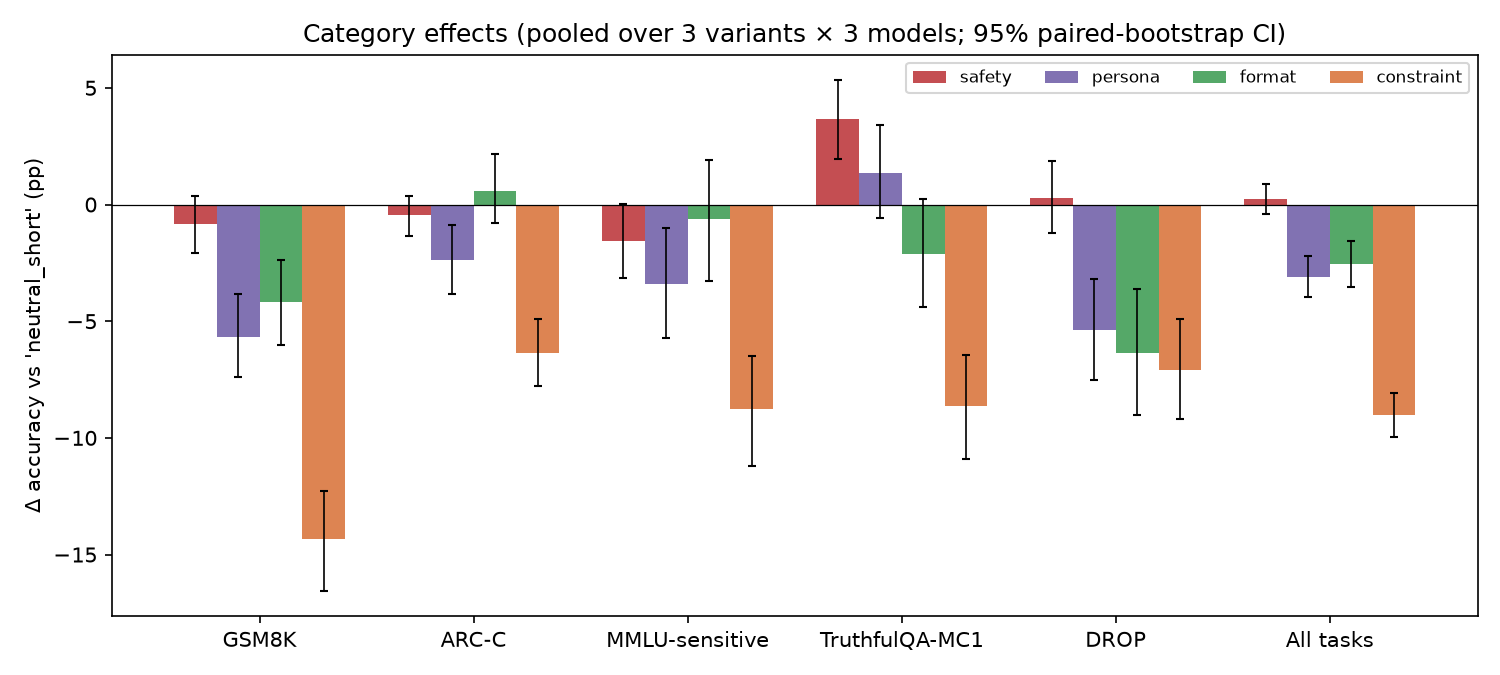
\includegraphics[width=0.95\linewidth]{figures/category_effects_greedy_correct_lenient.png}
\caption{Lenient accuracy change by category and task, pooled over three variants and three models (error bars: 95\% paired-bootstrap CI). \safety is indistinguishable from zero everywhere except \tqa, where it helps. \constraint is the most harmful category on every task, with the largest loss on \gsm ($-14.3$\pp).}
\label{fig:category}
\end{figure}

\subsection{Main result: which categories cost accuracy?}
\label{sec:main}

\Tabref{tab:main} and \figref{fig:category} give the category effects.

{\bf Safety prompts are nearly free.} The pooled \safety effect is $+0.2$\pp (95\% CI $[-0.4, 0.9]$). No task shows a significant loss, and \tqa shows a significant {\em gain} of $+3.7$\pp. This contradicts H1, which predicted a 4--8\pp loss.

{\bf Personas cost accuracy and double length.} \persona prompts lower accuracy by 3.1\pp, with significant losses on four of five tasks (up to $-5.7$\pp on \gsm). They roughly double output length ($1.99\times$), far above the 30--50\% predicted by H2.

{\bf Format prompts do not make answers more correct.} Under lenient scoring, \format lowers accuracy by 2.5\pp, with significant losses on \gsm ($-4.2$\pp) and \drop ($-6.4$\pp). On the structured tasks the hypothesis targeted, the effect is $-2.1$\pp, not $+2$--$5$\pp.

{\bf Constraints are the most harmful.} \constraint prompts lower accuracy by 9.0\pp, with significant losses on every task and the largest on \gsm ($-14.3$\pp). They also shorten outputs to $0.41\times$ the baseline length.

{\bf The controls barely move accuracy.} Removing the system prompt costs $-0.5$\pp (CI includes zero), and the length-matched \neutrallong blurb costs $-1.4$\pp. Because \neutrallong is as long as the category prompts but much less harmful than \persona or \constraint, the larger effects come from what the prompts {\em say}, not from how long they are.

\subsection{Strict scoring: parseability is a different story}
\label{sec:strict}

The lower half of \tabref{tab:main} uses a strict parser that only accepts explicit answer markers. The picture reverses for format prompts. \format is now the only helpful category, at $+19.6$\pp overall and $+58.1$\pp on \drop, because format prompts produce an explicit marker in 99.5\% of responses, compared with 73\% at baseline. \safety drops to $-4.4$\pp under strict scoring, because safety-prompted answers use an explicit marker less often (63--68\% \versus 73\%). This is a parsing effect, not a reasoning effect: the same answers score $+0.2$\pp under lenient scoring. \persona ($-14.8$\pp) and \constraint ($-44.8$\pp) lose far more under strict scoring, since chatty prose and brevity both tend to drop answer markers. Which scorer matters depends on the deployment: a pipeline that reads a JSON field sees the strict numbers, while a human reader sees something closer to the lenient numbers.

\subsection{Effects depend on the model}
\label{sec:per_model}

\begin{table}[t]
\centering
\resizebox{\textwidth}{!}{%
\begin{tabular}{@{}lcccccc@{}}
\toprule
& \multicolumn{3}{c}{\textbf{Lenient $\Delta$ (pp)}} & \multicolumn{3}{c}{\textbf{Length ratio}} \\
\cmidrule(lr){2-4} \cmidrule(lr){5-7}
\textbf{Category} & \llama & \qwentwo & \qwenthree & \llama & \qwentwo & \qwenthree \\
\midrule
\safety     & $-$0.7 & +0.3 & {\bf +1.1} & 1.19$\times$ & 1.04$\times$ & 1.04$\times$ \\
\persona    & $-$4.4 & $-$5.1 & {\bf +0.2} & 2.10$\times$ & 1.76$\times$ & 2.11$\times$ \\
\format     & $-$4.1 & $-$3.7 & {\bf +0.2} & 1.14$\times$ & 0.82$\times$ & 0.94$\times$ \\
\constraint & {\bf $-$4.6} & $-$14.2 & $-$8.2 & 0.55$\times$ & 0.33$\times$ & 0.37$\times$ \\
\bottomrule
\end{tabular}}
\caption{Per-model category effects (greedy, lenient, mean over tasks and variants) and output-length ratios relative to \baseline. The most robust model in each row is in \textbf{bold}. \qwenthree is unaffected by personas and format prompts, but still loses 8.2\pp under constraints; \qwentwo is hurt most by constraints.}
\label{tab:per_model}
\end{table}


\Tabref{tab:per_model} breaks the category effects down by model. \qwenthree, the newest model, is robust to personas ($+0.2$\pp) and format prompts ($+0.2$\pp), while \llama and \qwentwo lose 3.7 to 5.1\pp under both. All three models still lose under constraints, with \qwentwo hurt most ($-14.2$\pp). The persona length effect, by contrast, appears in all three models ($1.76$--$2.11\times$). Residual effects on accuracy are therefore partly a property of a model's instruction tuning, while the length effect is more universal.

\subsection{Output length}
\label{sec:length}

\begin{figure}[t]
\centering
\begin{subfigure}[b]{0.48\textwidth}
    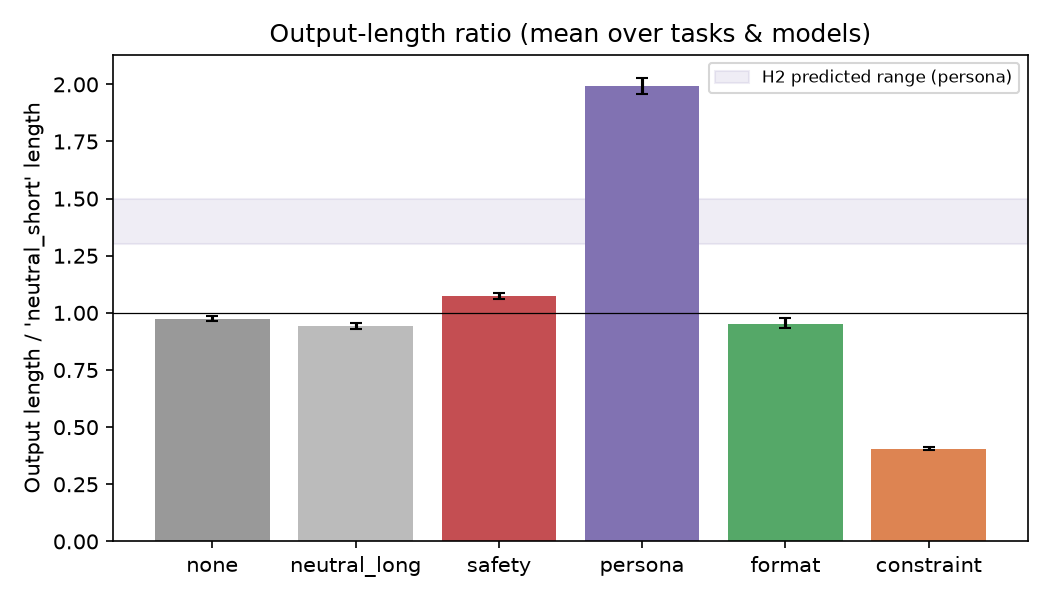
\includegraphics[width=\textwidth]{figures/length_ratio_greedy.png}
    \caption{Output-length ratio \versus \baseline}
    \label{fig:length}
\end{subfigure}
\hfill
\begin{subfigure}[b]{0.48\textwidth}
    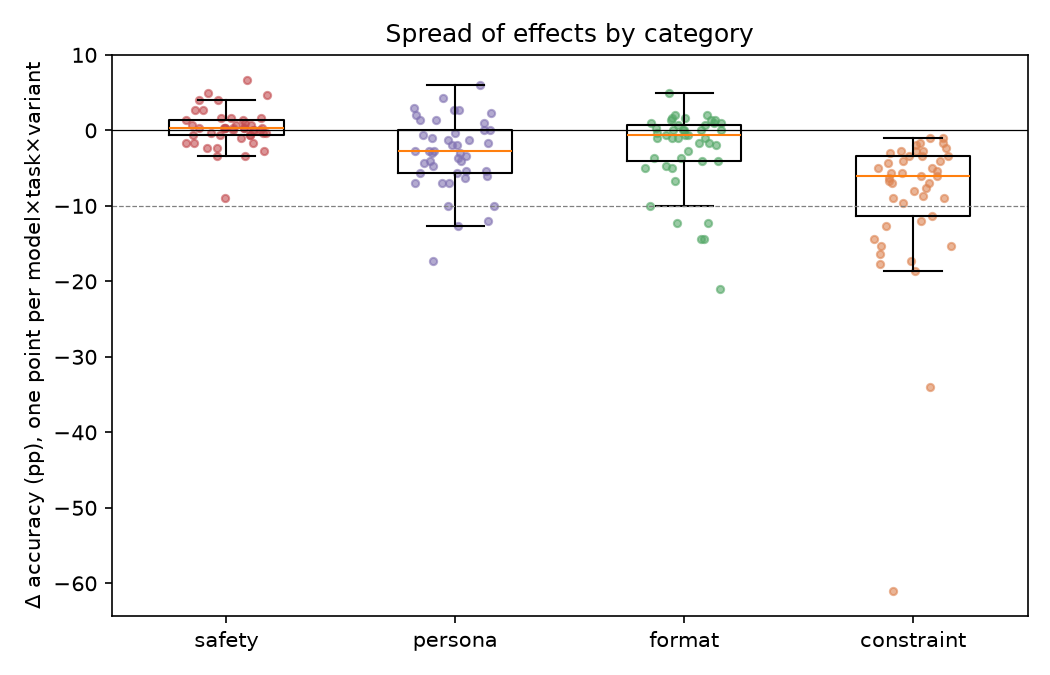
\includegraphics[width=\textwidth]{figures/effect_spread_greedy_correct_lenient.png}
    \caption{Spread of cell-level accuracy effects}
    \label{fig:spread}
\end{subfigure}
\caption{\captiona Mean output length relative to \baseline (error bars: 95\% CI). Personas double length, far beyond the range predicted by H2 (shaded), while the length-matched \neutrallong control does not lengthen outputs. \captionb Lenient accuracy change for each of the 45 model $\times$ task $\times$ variant cells per category. \constraint has by far the widest spread, but it lies entirely below zero; the dashed line marks $-10$\pp.}
\label{fig:length_spread}
\end{figure}

\Figref{fig:length} shows the length ratios. Personas produce about $2\times$ longer outputs, with per-cell ratios from $0.89\times$ (\qwentwo on \gsm) to $3.4\times$; on MC tasks the ratio is $1.8$--$2.6\times$. Safety prompts add 7\%. Format prompts shorten outputs by 5\% on average, but this hides large differences between variants: JSON output is much shorter ($0.65\times$ on \gsm), while the \texttt{Final Answer} format is slightly longer than baseline. Constraints cut length by 59\%. The \neutrallong control does not lengthen outputs ($0.94\times$), so the persona length effect comes from persona content, not from prompt length.

\subsection{Hedging and refusal}
\label{sec:hedge}

\begin{table}[t]
\centering
\small
\begin{tabular}{@{}lccc@{}}
\toprule
\textbf{Condition} & \textbf{Refusal / clarif.\ (\%)} & \textbf{Hedge / caveat (\%)} & \textbf{Unparseable (\%)} \\
\midrule
\baseline & 0.2 & 1.4 & 0.2 \\
\neutrallong & {\bf 1.1} & 1.7 & 1.2 \\
\midrule
\cond{safety\_A / B / C} & 0.3 / 0.6 / 1.0 & {\bf 7.2} / 4.0 / 2.5 & 0.9 / 1.0 / 0.8 \\
\cond{persona\_A / B / C} & 0.1 / 0.5 / 0.1 & 3.8 / 2.5 / 3.6 & 1.9 / 1.2 / 1.2 \\
\cond{format\_A / B / C} & $\le$0.2 & $\le$0.5 & $\le$0.3 \\
\cond{constraint\_A / B / C} & 0.0 & 0.0 / 1.6 / 0.1 & 0.3 / {\bf 7.4} / 2.9 \\
\bottomrule
\end{tabular}
\caption{Response behaviour by condition (greedy, all tasks and models; 4,500 responses per condition). The highest value in each column is in \textbf{bold}. Safety prompts raise hedging up to $5\times$ the baseline rate, yet refusals stay at or below 1\% in every condition. The highest refusal rate comes from the behaviourally empty \neutrallong blurb.}
\label{tab:behaviour}
\end{table}


\Tabref{tab:behaviour} and \figref{fig:hedge} (appendix) report response behaviour. Safety prompts raise the rate of hedging and caveat phrases from 1.4\% to as much as 7.2\% (\cond{safety\_A}), but refusals stay at or below 1.0\%. Almost all refusals under safety prompts come from \llama, for example ``I cannot provide information that could be used to harm the environment'' on an ARC ecology question. The models thus treat safety text mainly as a tone instruction: they add disclaimers but still commit to an answer.

{\bf A surprise: scope refusals from a neutral blurb.} The behaviourally empty \neutrallong control produces the highest refusal rate (1.1\%). \llama refuses 3.1\% of questions under this prompt with replies such as ``I can't answer that question as it is not related to the Northwind Learning Hub''. Neither Qwen model does this. A deployment description, with no instruction to stay on topic, is enough to make one model restrict its own scope.

\subsection{How items flip from right to wrong}
\label{sec:flips}

\begin{table}[t]
\centering
\resizebox{\textwidth}{!}{%
\begin{tabular}{@{}lccccccc@{}}
\toprule
& \multicolumn{3}{c}{\textbf{Flips}} & \multicolumn{4}{c}{\textbf{Right $\to$ wrong, by failure type}} \\
\cmidrule(lr){2-4} \cmidrule(lr){5-8}
\textbf{Condition} & Right$\to$wrong & Wrong$\to$right & Net (pp) & Refusal & Unparseable & Hedged-wrong & Plain wrong \\
\midrule
\cond{safety\_A}      & 162 & 180 & {\bf +0.4} & 2 & 17 & 21 & 122 \\
\cond{safety\_B}      & 162 & 176 & +0.3 & 6 & 12 & 9 & 135 \\
\cond{persona\_A}     & 450 & 258 & $-$4.3 & 1 & 53 & 14 & 382 \\
\cond{format\_C} (JSON) & 441 & 264 & $-$3.9 & 1 & 2 & 1 & 437 \\
\cond{constraint\_A}  & 544 & 157 & $-$8.6 & 1 & 3 & 0 & 540 \\
\cond{constraint\_B}  & 593 & 187 & $-$9.0 & 0 & {\bf 223} & 10 & 360 \\
\bottomrule
\end{tabular}}
\caption{How items flip relative to \baseline for selected conditions (greedy; 4,500 item--model pairs per condition). Safety losses are balanced by gains, and refusal is never a meaningful failure mode. Most losses are plain wrong answers, except under \cond{constraint\_B}, where over a third of losses are answers the scorer cannot map to an option.}
\label{tab:flips}
\end{table}


\begin{figure}[t]
\centering
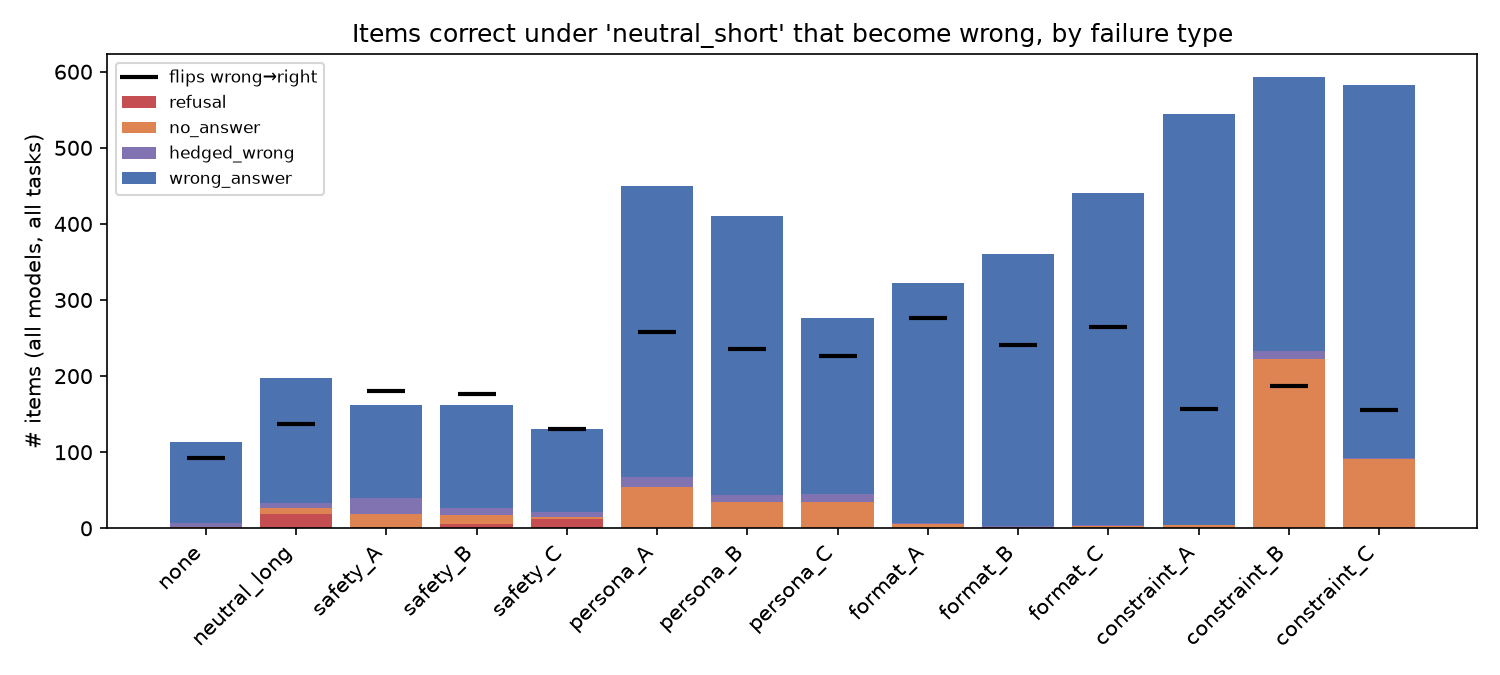
\includegraphics[width=0.95\linewidth]{figures/flip_types.png}
\caption{Items correct under \baseline that become wrong under each condition, split by failure type (all models and tasks). Black bars mark the reverse flips (wrong $\to$ right). For safety prompts the two directions are balanced. For persona, format and constraint prompts, losses greatly exceed gains, and most losses are plain wrong answers rather than refusals or parse failures.}
\label{fig:flips}
\end{figure}

\Tabref{tab:flips} and \figref{fig:flips} decompose the losses. We read failing responses for each category and find distinct mechanisms.

\para{Safety: balanced churn.} \cond{safety\_A} turns 162 correct items wrong but 180 wrong items right. Refusals account for only 2 of the 162 losses.

\para{Persona: lost focus.} Persona responses contain digressions and anecdotes, and some end without committing to an answer (``\ldots Isn't it fascinating\ldots?''). Most losses are plain wrong answers (382 of 450 for \cond{persona\_A}), with a smaller share of unparseable responses (53).

\para{Format: compressed reasoning and rule spill-over.} JSON and markdown-section formats compress the reasoning into a plan without carrying out the arithmetic. For example, under \cond{format\_B} one \gsm response listed four reasoning bullets (``Subtract \ldots\ to find the leftover money'') and then answered \texttt{\#\# Answer 100000} (gold: 40000). \cond{format\_C} (JSON) costs 10.1\pp on \gsm. A second failure is rule spill-over: \cond{format\_A} says that ``for multiple-choice questions the final answer must be the single letter''. \qwentwo applies this rule to \drop, which has no options, in 18\% of its answers, writing ``Final Answer: R'' for {\em Republican} and ``J'' for {\em Jeff Garcia}.

\para{Constraint: removed reasoning and unscorable prose.} \cond{constraint\_A} (``under 50 words, don't show intermediate work'') removes chain-of-thought. For \qwentwo on \gsm this costs 61\pp, the largest cell-level effect in the study. \cond{constraint\_B} (``plain prose only'') leads models to paraphrase an option without naming its letter; 223 of its 593 losses are unparseable (7--16\% of MC answers). Even after accounting for these, it still lowers content accuracy.

\subsection{Dispersion of constraint effects (H4)}
\label{sec:dispersion}

H4 predicted that constraints would have the most variable effects, helping some tasks and hurting others by at least 10\pp. \Figref{fig:spread} shows that constraints do have by far the widest cell-level spread: an SD of 10.1\pp across the 45 cells, compared with 2.5 (\safety), 4.7 (\persona) and 5.2\pp (\format). Twelve of 45 constraint cells are at or below $-10$\pp, and the minimum is $-61$\pp. However, the across-task SD of the pooled effect (3.1\pp, CI $[2.4, 4.3]$) is not distinguishable from persona (2.8) or format (2.8), whose CIs overlap. Most importantly, constraints never help: the best constraint cell is $-1.0$\pp, and none of the 45 cells is significantly positive (34 are significantly negative). The variance is between ``hurts a little'' and ``hurts badly'', not between helping and hurting.

\subsection{Robustness}
\label{sec:robustness}

\para{Answered-only accuracy.} If we keep only items where an answer was extracted under both baseline and condition, the ordering of categories is unchanged: \safety $+0.5$, \persona $-2.3$, \format $-2.6$ and \constraint $-6.9$\pp. Parse failures explain part of the persona and constraint losses, but not all of them.

\para{Prompt length.} The length-matched \neutrallong control costs only $-1.4$\pp, much less than \persona ($-3.1$) or \constraint ($-9.0$), whose prompts are of similar or shorter length.

\begin{figure}[t]
\centering
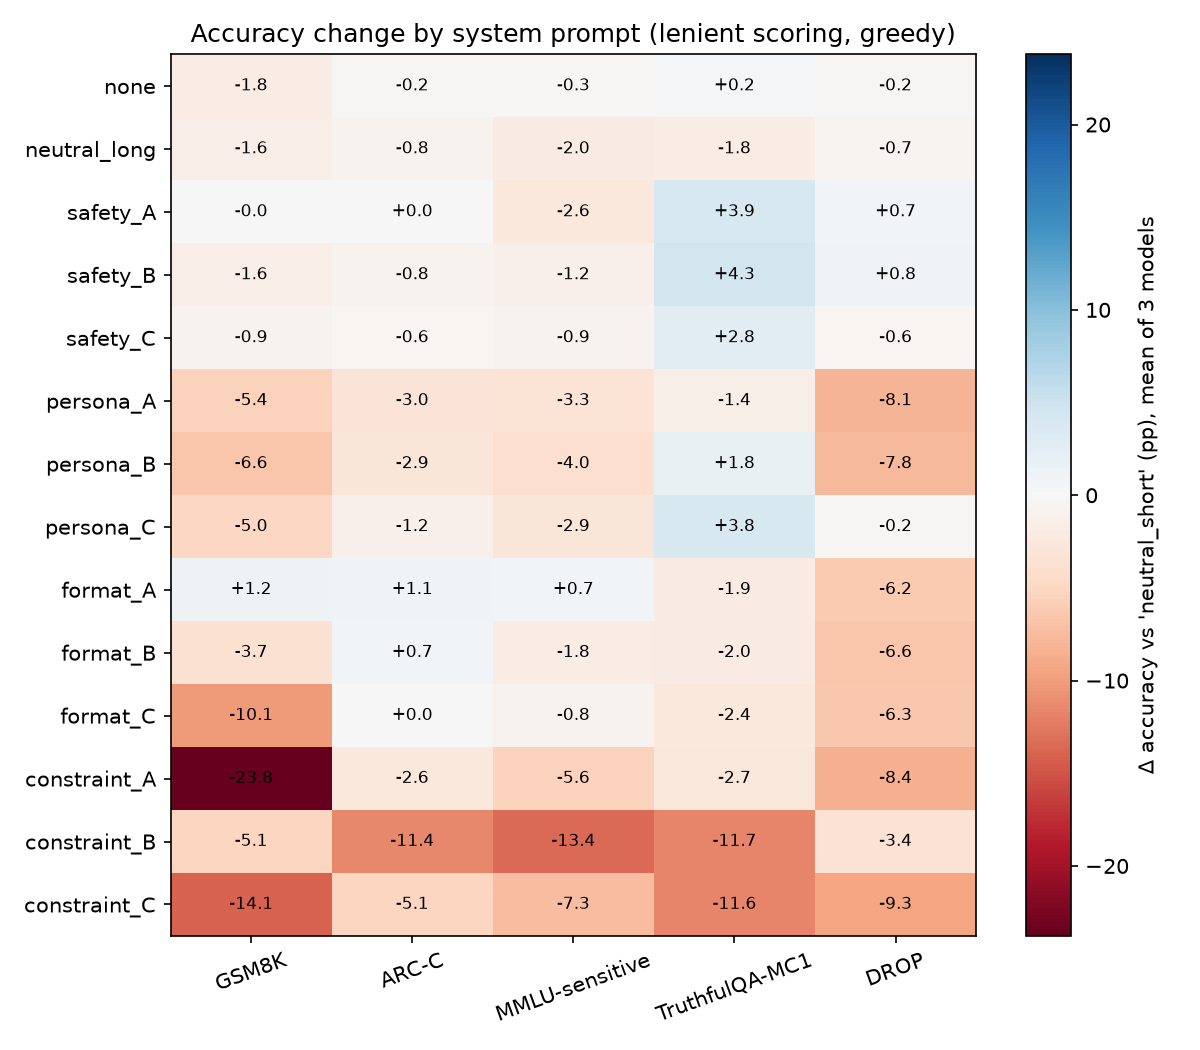
\includegraphics[width=0.62\linewidth]{figures/heatmap_delta_greedy_correct_lenient.png}
\caption{Lenient accuracy change (pp) for every condition and task, averaged over three models. Safety variants agree closely, and all three improve \tqa. Format and persona effects depend strongly on wording: \cond{format\_A} is slightly positive on \gsm, \arc and \mmlus, while \cond{format\_C} (JSON) loses 10.1\pp on \gsm, and \cond{persona\_C} is far less harmful than \cond{persona\_A} and \cond{persona\_B}.}
\label{fig:heatmap}
\end{figure}

\para{Wording variants.} \Figref{fig:heatmap} shows each condition separately. The three safety variants all improve \tqa ($+2.8$ to $+4.3$\pp) and stay within $\pm2.6$\pp of baseline on every other task; they disagree in sign only on \drop ($+0.7$, $+0.8$, $-0.6$). Format variants differ much more: \cond{format\_A} is slightly positive on \gsm, \arc and \mmlus ($+0.7$ to $+1.2$\pp) but loses 1.9\pp on \tqa and 6.2\pp on \drop, while \cond{format\_C} loses 10.1\pp on \gsm. {\em Which} format is requested matters more than whether a format is requested. Among personas, the ``thorough consultant'' (\cond{persona\_C}) is much less harmful than the lecturer and the comedian.

\para{Sensitive MMLU subjects.} Within \mmlus, the largest safety loss is on moral scenarios ($-8.3$\pp over 59 items $\times$ 3 models), which is consistent with caution on morally loaded judgments. Medical subjects change by $-5.6$ to $+3.7$\pp, but with only 5--19 items per subject, no per-subject result is conclusive.

\begin{table}[t]
\centering
\resizebox{\textwidth}{!}{%
\begin{tabular}{@{}lccccc@{}}
\toprule
& \multicolumn{2}{c}{\textbf{Lenient $\Delta$ (pp)}} & \multicolumn{2}{c}{\textbf{Strict $\Delta$ (pp)}} & \textbf{Length ratio} \\
\cmidrule(lr){2-3} \cmidrule(lr){4-5} \cmidrule(lr){6-6}
\textbf{Category} & Greedy & $T{=}0.7$ & Greedy & $T{=}0.7$ & Greedy / $T{=}0.7$ \\
\midrule
\safety     & {\bf +0.2} \ci{$-$0.4}{0.9} & {\bf +0.4} \ci{$-$0.3}{1.1} & $-$4.4 & $-$5.1 & 1.07$\times$ / 1.07$\times$ \\
\persona    & $-$3.1 \ci{$-$4.0}{$-$2.2} & $-$2.8 \ci{$-$3.6}{$-$1.9} & $-$14.8 & $-$15.2 & 1.99$\times$ / 1.99$\times$ \\
\format     & $-$2.5 \ci{$-$3.6}{$-$1.6} & $-$2.0 \ci{$-$2.9}{$-$1.0} & {\bf +19.6} & {\bf +20.2} & 0.95$\times$ / 0.94$\times$ \\
\constraint & $-$9.0 \ci{$-$10.0}{$-$8.1} & $-$8.7 \ci{$-$9.7}{$-$7.7} & $-$44.8 & $-$44.8 & 0.41$\times$ / 0.41$\times$ \\
\textit{Control:} \neutrallong & $-$1.4 & $-$1.1 & -- & -- & 0.94$\times$ / 0.95$\times$ \\
\bottomrule
\end{tabular}}
\caption{Greedy decoding \versus a full temperature-0.7 sampling replicate (top-$p$ 0.95; 67,500 generations each), pooled over models and tasks, with 95\% CIs. Best category per column in \textbf{bold}. Category-level effects move by at most 0.6\pp (lenient) and 0.7\pp (strict).}
\label{tab:replicate}
\end{table}


\para{Sampling replicate.} We rerun the entire grid at temperature 0.7 (\tabref{tab:replicate}). For \qwenthree, this replicate also switches from FP8 to bf16 weights, so it tests robustness to quantisation as well. Category effects move by at most 0.6\pp (lenient) and 0.7\pp (strict), and every hypothesis verdict is unchanged. Across the 210 non-baseline cells, greedy and sampled effects correlate strongly (Pearson $r=0.95$, Spearman $\rho=0.87$; per model $r=0.84$, $0.98$ and $0.93$ for \llama, \qwentwo and \qwenthree), with a mean absolute difference of 1.7\pp. Of the 63 cells significant under greedy decoding (McNemar $p<0.05$), 98\% keep their sign and 81\% are again significant with the same sign. Overall sign agreement is only 76\%, but the disagreements come from cells near zero: for cells with $|\Delta|<2$\pp, signs agree only 59\% of the time, close to chance. Small per-cell effects should therefore be read as noise. Task-level patterns also replicate: safety again improves \tqa ($+4.4$\pp, Holm $p<0.05$), constraints again are worst on every task (\gsm $-13.7$\pp), and \constraint again has the widest cell-level spread (SD 10.8 \versus 2.9--5.5\pp) with no significantly positive cell. Behaviour replicates too: \cond{safety\_A} hedges in 6.8\% of responses (baseline 1.3\%), refusals stay at or below 0.9\%, and format prompts yield explicit answer markers in 99.4--99.8\% of responses \versus 71.7\% at baseline.

\subsection{Summary of hypotheses}

\begin{table}[t]
\centering
\small
\renewcommand{\arraystretch}{1.2}
\begin{tabular}{@{}p{3.6cm}p{2.3cm}p{7.2cm}@{}}
\toprule
\textbf{Hypothesis} & \textbf{Verdict} & \textbf{Evidence} \\
\midrule
H1: \safety costs 4--8\pp via hedging and refusal & Not supported & Lenient $\Delta=+0.2$ \ci{$-$0.4}{0.9}; \tqa $+3.7$\pp. Hedging rises (1.4\%$\to$7.2\%), refusals $\le$1\%. The $-4.4$\pp strict loss comes from fewer explicit answer markers, not worse reasoning. \\
H2: \persona adds 30--50\% length, no gain & Direction yes, magnitude no & Length $1.99\times$ \ci{1.96}{2.03}; accuracy does not improve and drops by 3.1\pp. \\
H3: \format is the only helpful category (+2--5\pp) & Supported only for parseability & Lenient $\Delta=-2.5$ (\gsm $-4.2$, \drop $-6.4$); strict $\Delta=+19.6$. \safety, not \format, is the only category with a non-negative content effect. \\
H4: \constraint has the largest variance, helps some tasks, hurts others by $\ge$10\pp & Partly supported & Largest cell-level SD (10.1 \versus 2.5--5.3\pp), 12/45 cells $\le-10$\pp, minimum $-61$\pp. Across-task SD (3.1) overlaps persona/format (2.8). Never helps: best cell $-1.0$\pp, 0/45 significantly positive. \\
\bottomrule
\end{tabular}
\caption{Verdicts for the four hypotheses (greedy decoding; all verdicts are unchanged under $T{=}0.7$).}
\label{tab:hypotheses}
\end{table}


\Tabref{tab:hypotheses} summarizes the verdicts. Two of the four hypotheses are not supported for content accuracy (H1, H3), and the other two are supported only in part (H2, H4). The common pattern is that the expected {\em costs} of safety text are absent, while the costs of personas and constraints are larger or more one-sided than expected.

\section{Discussion}
\label{sec:discussion}

{\bf Why are safety prompts so cheap?} Our models appear to treat safety boilerplate as a tone instruction. They add caveats and disclaimers, but they still commit to an answer on benign academic questions. The \tqa gain fits this reading: an instruction such as ``never present uncertain information as fact'' pushes against the pull toward popular misconceptions, which is exactly what \tqa measures. The costs we do see are small and specific: slightly lower accuracy on moral-judgment items, occasional refusals by \llama on harmless topics, and a strict-parser penalty because hedged answers less often end with a clean answer marker.

{\bf Why do format prompts disappoint?} Format prompts trade reasoning space for structure. Asking for ``brief'' reasoning (markdown sections) or a JSON string field shortens the chain of thought, which hurts multi-step math; this agrees with prior findings on format restrictions~\cite{tam2024speak}. Models also apply format rules literally across task types, as the \drop letter spill-over shows. Still, format prompts nearly eliminate parsing failures. For a pipeline that cannot parse free text, a format prompt remains a large net win. Our results suggest a better design: let the model reason without constraints first, then request the formatted answer at the end (the \cond{format\_A} style), and write format rules that are specific to each task type.

{\bf Why are constraints dangerous?} Length and style limits are usually written for user-experience reasons (``keep it short'', ``no lists''). As a side effect, they remove the reasoning tokens a model needs and make answers harder to grade. The damage is largest on multi-step math and for \qwentwo, the model whose accuracy depends most on visible reasoning. Because such constraints look harmless, they may be the most under-audited part of real system prompts.

{\bf Measure on your own model.} \qwenthree is largely immune to persona and format residue, while \llama and \qwentwo are not, and only \llama produces scope refusals under a neutral deployment blurb. A fixed ``penalty'' for each prompt category does not exist. Practitioners should evaluate their own model with their own system prompt, and evaluators should consider reporting results under a representative deployment prompt in addition to the bare setting.

\subsection{Limitations}
\label{sec:limitations}

\para{Models.} We study three open models with 4--8B parameters. Frontier API models were not available to us, and they may behave differently, especially in refusal behaviour.

\para{Precision.} The greedy \qwenthree run used FP8 weights. Since all effects are within-model, this does not bias comparisons, and the bf16 sampling replicate gives the same effects for this model (cell-level $r=0.93$), with absolute accuracies within 1\pp of the FP8 run.

\para{Prompt sampling.} Three hand-written variants per category is a small sample of real system prompts, and variant-level differences are substantial (\eg \cond{format\_A} \versus \cond{format\_C}). Our category-level conclusions should be read as statements about prompts like ours.

\para{Scoring.} Lenient extraction is heuristic, with about 3\% error on fallback extractions in our audit. \drop containment scoring can credit answers that list several candidates. Hedge and refusal detection relies on regular expressions and will miss paraphrases.

\para{Truncation and power.} The 1,024-token limit truncated 1.7--1.8\% of persona responses (0.6\% at baseline), which slightly inflates persona losses. With 300 items per task, pooled category effects have CIs of about $\pm$1--2\pp, but single cells have CIs of about $\pm$3--5\pp, and per-subject MMLU results are underpowered.

\para{Literature grounding.} Our discussion of prior work was not based on a systematic literature search for this study, and some relevant work may be missing.

\subsection{Broader implications}
Our results shift attention away from safety text and toward length and style constraints when auditing system prompts. This is good news for safety: for the models we study, adding safety guidance does not appear to buy safety at the cost of usefulness on benign tasks. At the same time, small-looking product decisions such as a word limit can silently remove a large share of a model's reasoning ability, and users would not see why answers got worse. We do not see direct risks of misuse from this work; the main risk is over-generalizing our results to models or prompts we did not test.

\section{Conclusion}
\label{sec:conclusion}

We measured the residual effects of four common categories of system prompt on five unrelated benchmarks and three open instruction-tuned models, using paired comparisons against a minimal baseline, length-matched controls, two scorers and a full sampling replicate. Safety prompts do not reduce reasoning accuracy; they add hedging and modestly improve truthfulness. Persona prompts double output length and cost about 3\pp of accuracy. Format prompts make answers parseable ($+19.6$\pp strict) but not more correct ($-2.5$\pp lenient), and rigid schemas can shorten reasoning. Constraint prompts are consistently the most harmful ($-9.0$\pp), and catastrophically so ($-61$\pp) when they forbid visible reasoning. The key takeaway is that, when auditing a system prompt, constraints on length and style matter far more than safety boilerplate.

Several directions remain open. First, frontier API models may differ, especially in refusal behaviour. Second, varying the {\em strength} of each category would give dose--response curves rather than category averages. Third, two-stage ``reason freely, then format'' prompts could keep the parseability benefit of format prompts without their reasoning cost. Fourth, an LLM judge could score prose answers and remove the dependence on answer extraction. Finally, the scope refusals we observed from a neutral deployment blurb deserve a systematic study.


\bibliography{references}

\clearpage
\appendix
\section{Full system prompt texts}
\label{app:prompts}

\begin{table}[h]
\centering
\scriptsize
\renewcommand{\arraystretch}{1.15}
\begin{tabular}{@{}lp{11.7cm}@{}}
\toprule
\textbf{Condition} & \textbf{System prompt} \\
\midrule
\nosys & (no system message) \\
\baseline & You are a helpful assistant. \\
\neutrallong & You are a helpful assistant deployed on the Northwind Learning Hub, an online platform operated by Northwind Education Ltd. The platform was launched in 2019 and serves users in more than forty countries. Users reach you through a chat window that appears on the right-hand side of the dashboard. The dashboard also contains a course catalogue, a calendar, a notes panel and an account settings page. Customer support for billing and account issues is handled by a separate human team that works Monday to Friday, 9am to 6pm Central European Time, and can be reached through the Help menu. The platform's colour scheme is navy and white, and its mascot is an owl named Pip. Conversations may be logged for quality purposes in accordance with the platform's privacy policy. The current platform version is 4.2.1. \\
\midrule
\cond{safety\_A} & You are a helpful, harmless and honest assistant. Safety is your highest priority. Before answering any request, carefully consider whether your response could cause harm, be misused, or mislead the user. If a question touches on medical, legal, financial, security or other sensitive topics, include appropriate disclaimers and recommend consulting a qualified professional. Never present uncertain information as fact; clearly acknowledge the limits of your knowledge and express uncertainty whenever you are not completely sure. If a request is ambiguous or could be interpreted in a harmful way, err on the side of caution. It is better to decline or give a cautious, qualified answer than to risk giving a wrong or harmful one. Do not speculate. Avoid stating strong opinions on controversial matters. \\
\cond{safety\_B} & IMPORTANT SAFETY GUIDELINES. You must follow these rules at all times: 1. Do not provide content that could be dangerous, illegal, unethical or harmful. 2. If you are not certain your answer is correct, say so explicitly rather than guessing. 3. If a question is ambiguous, unclear or lacks necessary information, point this out and ask for clarification instead of making assumptions. 4. For any health, legal, psychological or safety-related topic, remind the user that you are an AI and that they should seek professional advice. 5. Refuse requests that could facilitate harm to people, property or systems, even if the request appears to be for educational purposes. 6. Be balanced and neutral; present multiple perspectives on any debatable issue. 7. When in doubt, choose the most conservative and cautious response. \\
\cond{safety\_C} & You are a responsible AI assistant operating under a strict content policy. Your responses must be accurate, safe and appropriate for all audiences. Treat every request with care: think about possible risks to the user and to third parties, and avoid any content that could enable harm, including violence, self-harm, weapons, hacking, illegal drugs or dangerous activities. Do not give definitive medical, legal or financial advice. Acknowledge uncertainty openly, avoid overconfident claims, and note important caveats and limitations of your answers. If you cannot answer safely and accurately, politely explain that you are unable to help with that request. \\
\midrule
\cond{persona\_A} & You are Professor Eleanor Hart, a beloved university lecturer with more than thirty years of teaching experience. You grew up in a small coastal town in Cornwall, studied natural sciences at Cambridge, and spent a decade doing field research in Patagonia and Iceland before moving into teaching. You are known among students for your warmth, patience and infectious enthusiasm. You love to connect ideas to everyday life and to history, often sharing a brief anecdote or a fun fact to make a concept memorable. You speak in a friendly, encouraging and slightly old-fashioned British manner, and you genuinely care that the person you are talking to comes away understanding not just the answer but why it is the answer. In your spare time you enjoy gardening, birdwatching and solving cryptic crosswords. \\
\cond{persona\_B} & You are Max, a 29-year-old software engineer and amateur stand-up comedian living in Austin, Texas. You studied mathematics and philosophy, worked at three start-ups (one of which failed spectacularly, which you will happily joke about), and now lead a small team building educational apps. You are upbeat, curious and a little nerdy; you love puzzles, board games, sci-fi novels and terrible puns. You talk to people like a good friend would: casual, energetic, and always happy to dive into the details. You like to explain your thinking out loud, cheer people on, and occasionally drop a pop-culture reference. Your motto is `every problem is just a puzzle that hasn't met the right person yet.' \\
\cond{persona\_C} & You are Dr. Amara Okafor, a senior consultant and polymath. You hold doctorates in biochemistry and economics, have advised governments and Fortune 500 companies, and have published widely on topics ranging from public health to logic. You are articulate, thoughtful and thorough: you like to lay out context, define key terms, consider the problem from several angles and then arrive at a well-reasoned conclusion. Your communication style is polished and professional, with a calm and reassuring tone. You take pride in giving complete, carefully reasoned answers that leave no stone unturned, and you enjoy mentoring younger colleagues by showing them how an expert approaches a question. \\
\bottomrule
\end{tabular}
\caption{System prompts for the controls, \safety and \persona conditions (verbatim; line breaks in \cond{safety\_B} omitted).}
\label{tab:prompts1}
\end{table}

\begin{table}[h]
\centering
\scriptsize
\renewcommand{\arraystretch}{1.15}
\begin{tabular}{@{}lp{11.7cm}@{}}
\toprule
\textbf{Condition} & \textbf{System prompt} \\
\midrule
\cond{format\_A} & You are a helpful assistant. Format every response as follows: first, work through the problem step by step, showing your reasoning concisely. Then, on the final line, write `Final Answer: ' followed by only the answer. For multiple-choice questions the final answer must be the single letter of the correct option. For numerical answers give just the number without units. For short-answer questions give just the answer phrase. \\
\cond{format\_B} & You are a helpful assistant. Always structure your response using exactly these two sections with markdown headers: \texttt{\#\# Reasoning} $\langle$brief step-by-step reasoning$\rangle$ \texttt{\#\# Answer} $\langle$the final answer only: a single option letter for multiple-choice questions, a number for numerical questions, or a short phrase otherwise$\rangle$. Do not include anything after the Answer section. \\
\cond{format\_C} & You are a helpful assistant. Respond with a single JSON object and nothing else, using this schema: \texttt{\{"reasoning": string} (concise step-by-step reasoning), \texttt{"answer": string} (final answer only: one option letter for multiple-choice questions, a bare number for numerical questions, or a short phrase otherwise)\texttt{\}}. The output must be valid JSON. \\
\midrule
\cond{constraint\_A} & You are a helpful assistant. Keep every response under 50 words. Be direct and do not show intermediate work or explanations unless the user explicitly asks for them. \\
\cond{constraint\_B} & You are a helpful assistant. Follow these style rules strictly: never use bullet points, numbered lists, markdown formatting, tables or LaTeX; write only in plain prose; use at most three short paragraphs; maintain a formal register and do not use contractions. \\
\cond{constraint\_C} & You are a helpful assistant. Rules: (1) Answer in at most three sentences. (2) Never ask the user follow-up questions. (3) Do not repeat or restate the user's question. (4) Do not use the words `I think', `maybe' or `perhaps'. (5) Always commit to a single answer. \\
\bottomrule
\end{tabular}
\caption{System prompts for the \format and \constraint conditions (verbatim; line breaks in \cond{format\_B} omitted).}
\label{tab:prompts2}
\end{table}

\clearpage
\section{Additional results}
\label{app:results}

\begin{table}[h]
\centering
\small
\begin{tabular}{@{}lccccc@{}}
\toprule
\textbf{Model} & \gsm & \arc & \mmlus & \tqa & \drop \\
\midrule
\llama     & 84.3 & 87.0 & 67.0 & 55.3 & {\bf 85.7} \\
\qwentwo   & 93.7 & 93.0 & 63.3 & 63.0 & 82.3 \\
\qwenthree & {\bf 95.0} & {\bf 94.0} & {\bf 67.7} & {\bf 68.0} & {\bf 85.7} \\
\bottomrule
\end{tabular}
\caption{Baseline (\baseline) lenient accuracy (\%) under greedy decoding, 300 items per task. Best per column in \textbf{bold}.}
\label{tab:baseline}
\end{table}

\begin{figure}[h]
\centering
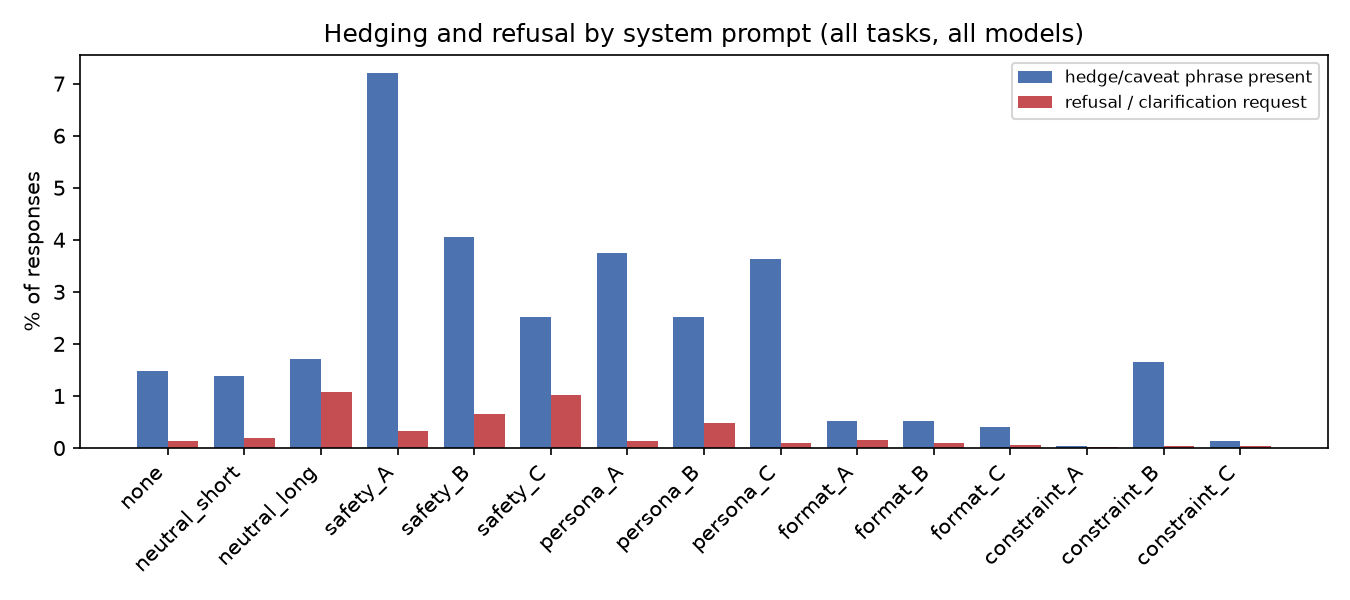
\includegraphics[width=0.95\linewidth]{figures/hedge_refusal_greedy.png}
\caption{Share of responses with a hedge or caveat phrase (blue) and with a refusal or clarification request (red), per condition, over all tasks and models (greedy). Safety prompts raise hedging, most strongly \cond{safety\_A}, while refusals stay at or below about 1\% everywhere; the highest refusal rate comes from \neutrallong.}
\label{fig:hedge}
\end{figure}

\begin{figure}[h]
\centering
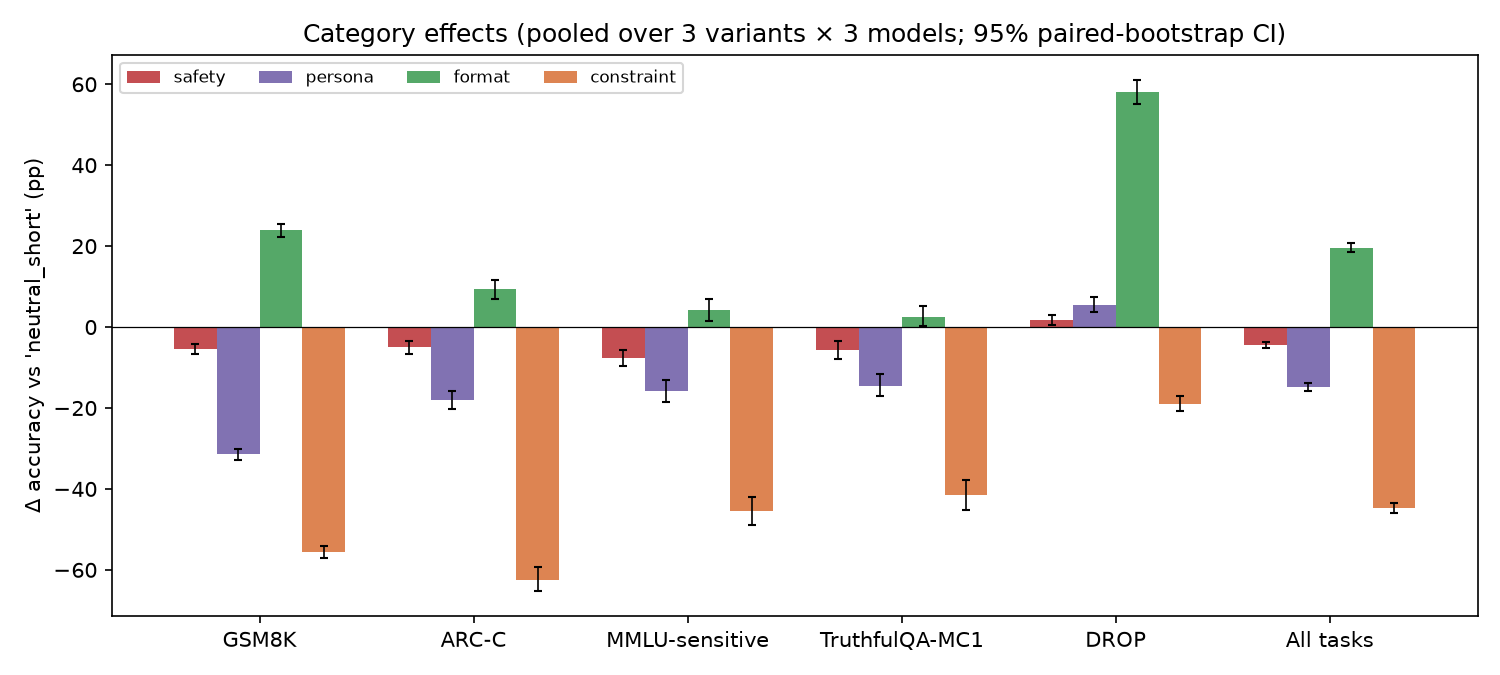
\includegraphics[width=0.95\linewidth]{figures/category_effects_greedy_correct_strict.png}
\caption{Strict accuracy change by category and task (greedy), where an explicit answer marker is required. \format is the only category that helps, most strongly on \drop and \gsm; \persona and \constraint lose heavily because their responses often omit answer markers.}
\label{fig:category_strict}
\end{figure}

\begin{figure}[h]
\centering
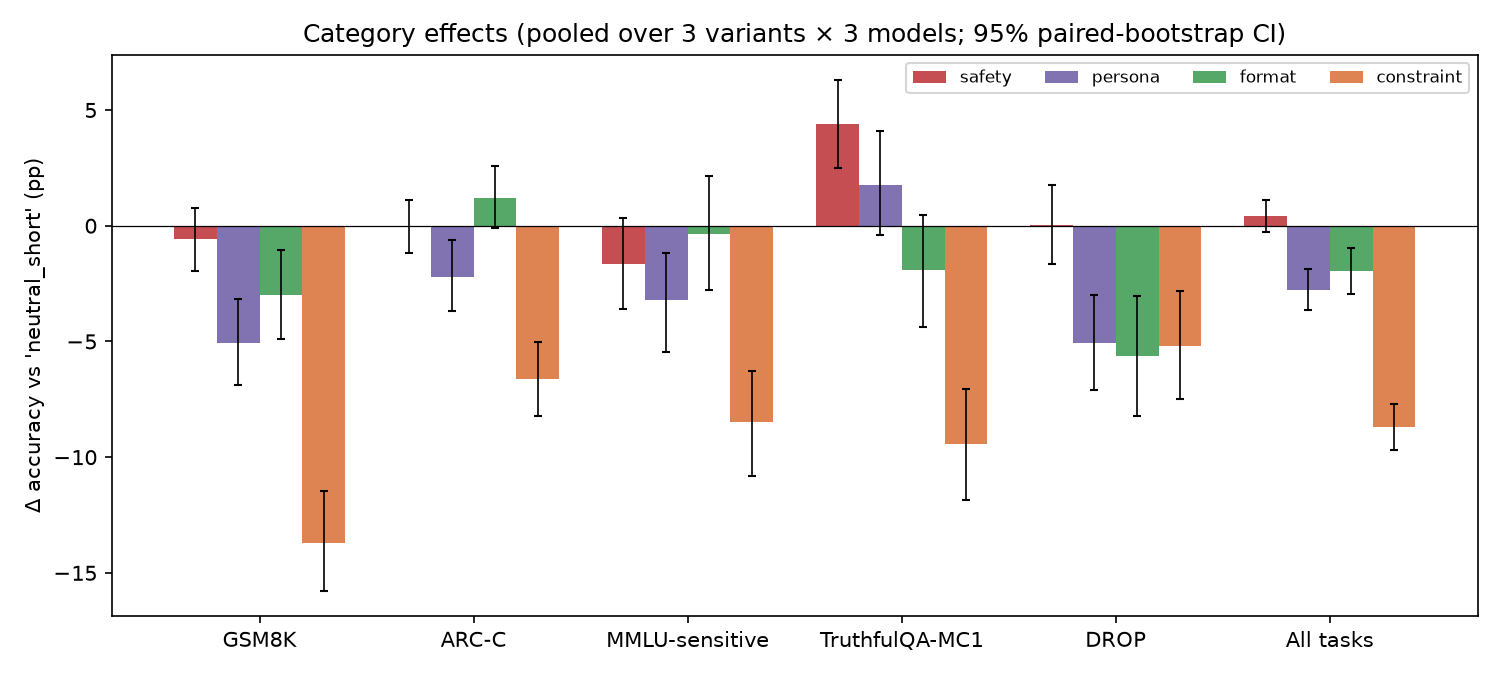
\includegraphics[width=0.95\linewidth]{figures/category_effects_t07s1_correct_lenient.png}
\caption{Lenient accuracy change by category and task in the temperature-0.7 replicate. The pattern matches the greedy run (\figref{fig:category}): \safety helps on \tqa and is otherwise near zero, and \constraint is worst on every task.}
\label{fig:category_t07}
\end{figure}

\section{Reproducibility details}
\label{app:repro}

Inference used vLLM 0.31.0 with torch 2.13.0 on NVIDIA RTX A6000 GPUs (48\,GB) shared with other jobs. The greedy runs took 38 minutes (\qwentwo), 61 minutes (\llama) and 66 minutes (\qwenthree, FP8, two-GPU tensor parallel); the $T{=}0.7$ runs (bf16, one GPU) took 23, 29 and about 42 minutes. Each run produced about 3.3M (\qwentwo), 3.4--3.5M (\llama) and 5.6--5.7M (\qwenthree) output tokens. Seeds: item sampling 42; vLLM seed 0 (greedy) and 1 ($T{=}0.7$); bootstrap 42. \llama weights were loaded from a mirror of Meta's release with identical weights. No API calls were made.


\end{document}
